\documentclass{article}

% Language setting
% Replace `english' with e.g. `spanish' to change the document language
\usepackage[english]{babel}

% Change the figure naming convention
\addto\captionsenglish{\renewcommand{\figurename}{Abb.}}

% Set page size and margins
% Replace `letterpaper' with `a4paper' for UK/EU standard size
\usepackage[letterpaper,top=2cm,bottom=2cm,left=3cm,right=3cm,marginparwidth=1.75cm]{geometry}

% Comments
\usepackage{verbatim}

% Useful packages
\usepackage{amsmath,amsthm,amssymb}
\usepackage{graphicx}
\usepackage[colorlinks=true, allcolors=blue]{hyperref}
\usepackage{tikz} % Positioning images

% Spacing
\frenchspacing

% Subfigures
\usepackage{subcaption}

% equation numbering includes section
\numberwithin{equation}{section} 

% Define macros
\newcommand{\authorname}{Yan-Xing Lan}
\newcommand{\subject}{Symmetrien und Projektionen – Invarianzphänomene bei Polyedern}

% Define definition 
\usepackage{tcolorbox}
\tcbuselibrary{theorems}
\theoremstyle{definition}
\newtheorem{definition}{Definition}
%\newtcbtheorem
%  []% init options
%  {definition}% name
%  {Definition}% title
%  {%
%    colback=green!5,
%    colframe=green!35!black,
%    fonttitle=\bfseries,
%  }% options
%  {def}% prefix

% Define examples
\theoremstyle{definition}
\newtheorem{example}{Beispiel}

% Define task
\newtheoremstyle{break}
  {\topsep}{\topsep}%
  {}{}%
  {\bfseries}{}%
  {\newline}{}%
\theoremstyle{break}
\newtheorem{exercise}{Aufgabe}

% Define theorem, lemma, proposition
\theoremstyle{plain}
\newtheorem{theorem}{Satz}
\newtheorem{proposition}{Proposition}
\newtheorem{lemma}{Lemma}



% Remove indent on whole document
\setlength{\parindent}{0pt}

\begin{document}

% Sicherstellen, dass man nicht auf den Seitenrand schreibt
\emergencystretch 3em

% -------------------------
% COVER PAGE
% -------------------------


\begin{titlepage}

    % Add image to top-left corner
    \begin{tikzpicture}[remember picture, overlay]
        node[anchor=north west, xshift=1cm, yshift=-1cm] at (current page.north west) {
        
\includegraphics[width=0.2\textwidth]{images/eth_logo_kurz_pos.png} 
    };
    \end{tikzpicture}

    
    {\centering
    \vspace*{2cm}
    {\Large \textbf{Mentorierte Arbeit in Fachwissenschaftlicher Vertiefung mit pädagogischem Fokus in Mathematik} \par}
    \vspace{0.5cm}
    {\Large zu \par}
    \vspace{0.5cm}
    {\Huge\bfseries \subject \par}
    \vspace{0.5cm}
    {\Large von \par}
    \vspace{0.5cm}
    {\Large \authorname \par}
    \vspace{1cm}
    }
    {
    \textbf{Inhalt} \newline
    Ziel dieser Arbeit ist es, eine Invarianzeigenschaft von symmetrischen Polyedern aufzuzeigen. Dabei wird diese Eigenschaft insbesondere an den regulären Tetraeder, Hexaeder und Ikosaeder betrachtet. 
    \vspace{1cm}
    
    \textbf{Zielpublikum}\newline
    Lerhpersonen
    \vspace{1cm}
    
    \textbf{Voraussetzungen}\newline
    Vorausgesetzt werden sowohl die komplexen Zahlen als auch grundlegende Begriff aus der Linearen Algebra, insbesondere Orthogonalprojektionen und die Darstellung von Abbildungen als Matrizen.
    \vspace{1cm}
    
    \textbf{Form}\newline
    Lesetext mit Aufgaben und Lösungen
    \vspace{1cm}
    
    %\textbf{Bearbeitungsdauer}\newline
    %Lore ipsum ... \newline
    %\vspace{1cm}
    
    \textbf{Betreuung}\newline
    Prof. Dr. Norbert Hungerbühler
    \vspace{1cm}

    \textbf{Datum}\newline
    \large \today\par
    }
\end{titlepage}

% -------------------------
% TITLE PAGE
% -------------------------
\title{\subject}
\author{\authorname}
\date{\today}
% Anpassung Inhaltverzeichnis Bezeichnung
\renewcommand*\contentsname{Inhaltsverzeichnis}
\setcounter{tocdepth}{2}
\maketitle

% -------------------------
% Content
% -------------------------

% Table of content
\newpage
\tableofcontents

% Chapters
\section{Einleitung}
In der vorliegenden Arbeit bereiten wir die Publikation \textit{Orthogonal Projections of Symmetric Polyhedra} von N. Hungerbühler und Y. Zhang \cite{hungerbuehler_symmetric_polyhedra} für ein breiteres Publikum auf. Die Zielgruppe umfasst unter anderem interessierte Schülerinnen und Schüler, Studierende sowie Lehrpersonen. Diese Arbeit führt die notwendige Theorie ein, um die zentralen Ideen und Berechnungen der Originalpublikation nachzuvollziehen. Im ersten Kapitel werden die grundlegenden Begriffe und Konzepte etabliert, während Kapitel \ref{sec:orthogonalprojektionen} den Beweis der Hauptaussage behandelt. Wir beginnen mit einem Einführungsbeispiel, das die Erkenntnisse der Publikation motivieren und veranschaulichen soll. Darauf folgt eine Einführung bzw. Repetition zu regulären Polyedern, Symmetriegruppen und Orthogonalprojektionen. Mit diesem theoretischen Fundament sind wir anschließend in der Lage, die mathematischen Aussagen in Kapitel \ref{sec:orthogonalprojektionen} fundiert zu beweisen.

 \subsection{Einführungsbeispiel}
Das zentrale Thema dieses Abschnitts sind Orthogonalprojektionen regulärer Polyeder auf Ebenen. Als Einstieg betrachten wir die Projektion eines Würfels auf eine Ebene im Raum. Der Würfel, auch \textbf{reguläres Hexaeder} genannt, siehe Abb. \ref{fig:einheitswürfel}, besitzt zahlreiche interessante Merkmale. Dazu gehören insbesondere seine Symmetrieeigenschaften, welche in Abschnitt \ref{sec:symmetrieeigenschaftwürfel} detailliert analysiert werden. Im Rahmen dieses Einführungsbeispiels fokussieren wir uns jedoch primär auf eine spezifische Eigenschaft der Kantenlängen der Orthogonalprojektion.

\begin{figure}[htp]
    \centering
    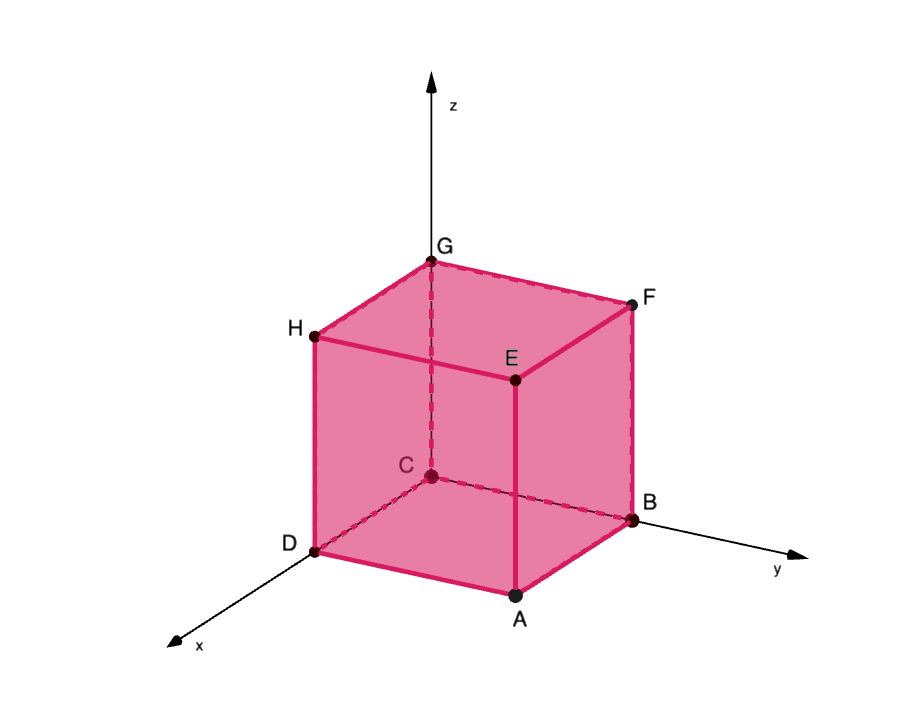
\includegraphics[width=0.7\textwidth, keepaspectratio]{images/einleitung/wuerfel_ortho_projektionen.png} 
    \caption{Regulärer Hexaeder $W$ mit Eckpunkten $A, B, \dots, H$.}
    \label{fig:einheitswürfel}
\end{figure}

Wir untersuchen, ob es eine invariante Eigenschaft in Bezug auf die projizierten Kantenlängen gibt. Eine Hypothese könnte lauten, dass die Summe der Längen aller projizierten Kanten eines Würfels bei einer Orthogonalprojektion unabhängig von der Lage der Projektionsebene ist. Um die Plausibilität dieser Hypothese zu prüfen, betrachten wir zunächst die Projektionen der Würfelkanten auf zwei verschiedene Ebenen. Sollte die Eigenschaft bereits für diese zwei Fälle nicht gelten, liesse sich die Hypothese direkt widerlegen. Das Nachvollziehen von Hypothesen an konkreten Instanzen ist zudem oftmals hilfreich, um ein besseres Verständnis aufzubauen und möglicherweise eine bessere Hypothese zu finden. Dieser Untersuchung gehen wir in Beispiel \ref{ex:wuerfelprojektionen} nach.



\begin{example}[Orthogonalprojektionen der Kanten eines Würfels auf eine Ebene] \label{ex:wuerfelprojektionen} 
Seien $E_1, E_2 \subset \mathbb{R}^3$ zwei Ebenen gegeben durch 

\begin{align}
    E_1:\ &x+y+z = 0,  \label{eq:ebene1}\\
    E_2:\ &x-y = 0 . \label{eq:ebene2}
\end{align}

 Sei $K_W$ die Menge der Kanten eines Würfels $W$, welcher in Abbildung \ref{fig:einheitswürfel} dargestellt ist. Wir wollen überprüfen, ob die Summe der Kantenlängen von einer Orthogonalprojektion auf diese beiden Ebenen identisch ist. Diese Behauptung kann wie folgt formuliert werden
\begin{align} \label{eq:hypothese1}
    \sum_{k \in K_W} \|\Pi_{E_1}(\vec{v}_k)\| = \sum_{k \in K_W} \|\Pi_{E_2}(\vec{v}_{k})\|,
\end{align}

wo $\Pi_{E_i}: \mathbb{R}^3 \rightarrow E_i$ die Orthogonalprojektion auf die Ebene $E_i \subset \mathbb{R}^3$ ist und $\vec{v}_k$ der zur Kante $k$ gehörende Richtungsvektor. Um diese Behauptung zu überprüfen, berechnen wir explizit die projizierten Kantenlängen eines regulären Hexaeders mit Kantenlänge $1$ und addieren diese auf. Diese Normierung vereinfacht die Rechnung, ohne die Allgemeingültigkeit einzuschränken, da die Ergebnisse für eine beliebige Kantenlänge $a$ lediglich um den Faktor $a$ skaliert würden. Die Ebene $E_1$, auf die wir projizieren, ist gegeben durch die Gleichung \eqref{eq:ebene1} mit dem Einheitsnormalenvektor 
\begin{align}
    \vec{n}_{E_1}  = \frac{1}{\sqrt{3}}\begin{pmatrix} 1 \\ 1 \\ 1 \end{pmatrix} .\nonumber
\end{align}

    \begin{figure}[htp]
    \centering
    \includegraphics[width=10cm]{images/einleitung/WürfelE1.png}
    \caption{Projektion der Kanten des Würfels auf die Ebene $E_1$ mit Normalenvektor $\vec{n}_{E_1}$.}
    \label{fig:würfelE1}
    \end{figure}

Bevor wir die Orthogonalprojektionen explizit berechnen, halten wir folgende Beobachtungen fest (siehe Abbildung \ref{fig:beobachtungenOrthogonalprojektionWurfel}):
\begin{itemize}
    \item Die Translation einer Strecke verändert die Länge ihrer Orthogonalprojektion auf eine Ebene nicht.
    \item Infolgedessen können wir jede Kante des Würfels als einen Vektor betrachten, indem wir ihren Fusspunkt in den Ursprung verschieben. 
\end{itemize}

    \begin{figure}[htp]
        \centering
        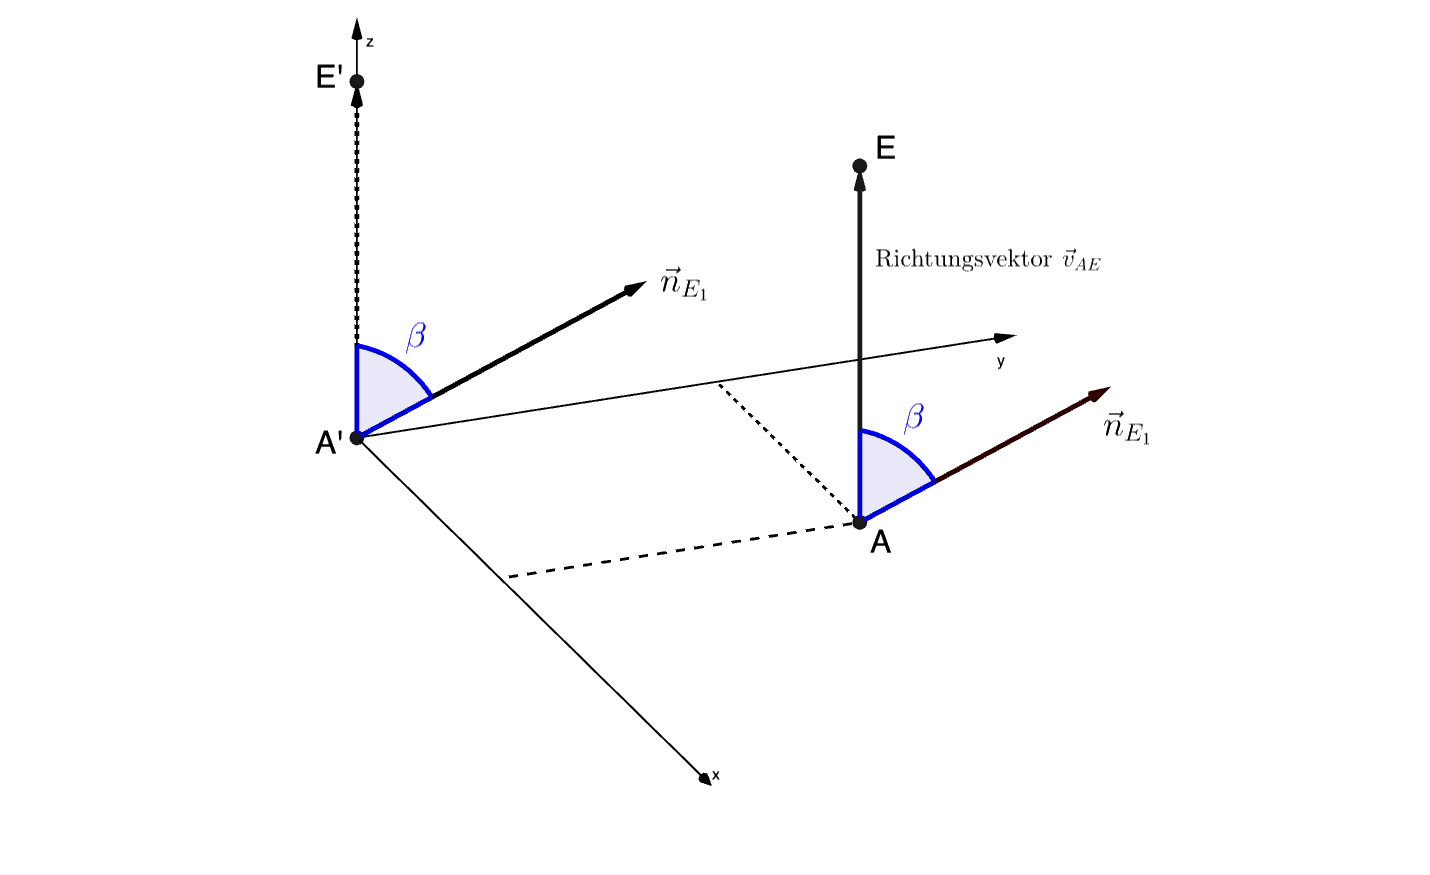
\includegraphics[width=10cm]{images/einleitung/VerschiebungKoordinatensystem.png}
        \caption{Beispiel der Translation des Richtungsvektors $\vec{v}_{AE}$. Der Winkel $\beta$ zum Normalenvektor $\vec{n}_{E_1}$ bleibt dabei erhalten.}
        \label{fig:beobachtungenOrthogonalprojektionWurfel}
    \end{figure}

Es lässt sich beobachten, dass die Strecken $\overline{CG}$, $\overline{CB}$ und $\overline{CD}$ den gleichen Winkel $\alpha$ mit dem Normalenvektor $\vec{n}_{E_1}$ einschliessen. Da alle Kanten des regulären Hexaeders zudem dieselbe Länge besitzen, sind auch ihre Projektionslängen identisch. Aus den vorangegangenen Überlegungen folgt, dass sämtliche Kanten des Würfels die gleiche Projektionslänge auf die Ebene $E_1$ aufweisen. Zur Berechnung dieser Länge können wir elementare trigonometrische Funktionen verwenden:

\begin{align} \label{eq:einführungsbeispielprojectionsimple}
    \|\Pi_{E_1}(\vec{v}_{CG})\| = \sin(\alpha) \cdot \|\vec{v}_{CG}\|,
\end{align}

wobei $\vec{v}_{CG}$ den Vektor der Kante $\overline{CG}$ repräsentiert und $\alpha$ der Winkel zwischen diesem Vektor und dem Normalenvektor $\vec{n}_{E_1}$ ist. Mit 
    \begin{align}
        \overline{CG}: \vec{v}_{CG}&=\begin{pmatrix} 0 \\ 0 \\ 1 \end{pmatrix},\|\vec{v}_{CG}\| = 1 \nonumber
    \end{align} sowie der Berechnungen
    \begin{align}
        \cos(\alpha) &= \frac{\vec{v}_{CG} \cdot \vec{n}_{E_1}}{\|\vec{v}_{CG}\| \|\vec{n}_{E_1}\|} = \frac{1}{\sqrt{3}} \nonumber \\
        \sin(\alpha) &= \sqrt{1-\cos^2(\alpha)} = \sqrt{\frac{2}{3}}, \nonumber
    \end{align}
    folgt aus Gleichung \eqref{eq:einführungsbeispielprojectionsimple}
    \begin{align}
        \|\Pi_{E_1}(\vec{v}_{CG})\| = \sqrt{\frac{2}{3}} \cdot 1= \sqrt{\frac{2}{3}} . \nonumber
    \end{align}
    Um die Summe aus Gleichung \eqref{eq:hypothese1} zu erhalten, müssen wir über alle Kanten in $K_W$ summieren und erhalten 
    \begin{align} \label{eq:summeebene1}
        \sum_{k \in K_W} \|\Pi_{E_1}(\vec{v}_{k})\| = 12 \cdot \sqrt{\frac{2}{3}} = 4\sqrt{6}.
    \end{align}
    
Wir behalten dieses Ergebnis im Hinterkopf und betrachten nun die Orthogonalprojektion auf die Ebene $E_2$ mit dem Einheitsnormalenvektor
    \begin{align}
        \vec{n}_{E_2} = \frac{1}{\sqrt{2}}\begin{pmatrix} 1 \\ -1 \\ 0 \end{pmatrix} .\nonumber
    \end{align}
    
    
    \begin{figure}[htp]
    \centering
    \includegraphics[width=0.7\textwidth, keepaspectratio]{images/einleitung/WürfelE2.png}
    \caption{Projektion der Kanten des Würfels auf die Ebene $E_2$ mit Normalenvektor $\vec{n}_{E_2}$.}
    \label{fig:würfelE2}
    \end{figure}
    
Aufgrund der Symmetrie des regulären Hexaeders können wir bei dieser Projektion zwei verschiedene Gruppen von Kanten unterscheiden:
\begin{itemize}
    \item Vier Kanten liegen parallel zur Ebene $E_2$ bzw. stehen orthogonal auf dem Normalenvektor $\vec{n}_{E_2}$, wie beispielsweise die Kante $\overline{CG}$.
    \item Die restlichen acht Kanten schliessen alle denselben Winkel $\alpha$, siehe Abbildung \ref{fig:würfelE2},mit dem Normalenvektor $\vec{n}_{E_2}$ ein, wie beispielsweise die Kante $\overline{GH}$.
\end{itemize}

Für die parallel zur Ebene $E_2$ verlaufenden Kanten gilt, dass ihre Länge bei der Projektion erhalten bleibt: 
\begin{align}
    \|\Pi_{E_2}(\vec{v}_{CG})\| = 1. \nonumber
\end{align}
    Für die anderen acht Kanten berechnen wir die Projektionslänge analog zu Gleichung \eqref{eq:einführungsbeispielprojectionsimple}. Da der Richtungsvektor $\vec{v}_{GH} = (1, 0, 0)^T$ einen Winkel von $\alpha = 45^\circ$ mit dem Normalenvektor $\vec{n}_{E_2}$ einschliesst, erhalten wir
\begin{align}
     \|\Pi_{E_2}(\vec{v}_{GH})\| = \sin\left(\frac{\pi}{4}\right) \cdot \|\vec{v}_{GH}\| = \frac{\sqrt{2}}{2} \cdot 1 = \frac{\sqrt{2}}{2}. \nonumber
\end{align}

Die Summation über alle 12 Kanten des regulären Hexaeders $W$ ergibt somit
\begin{align} \label{eq:summeebene2}
    \sum_{k \in K_W} \|\Pi_{E_2}(\vec{v}_k)\| = 4 \cdot 1 + 8 \cdot \frac{\sqrt{2}}{2} = 4 + 4\sqrt{2} = 4(1+\sqrt{2}).
\end{align}
Ein Vergleich der Ergebnisse aus den Gleichungen \eqref{eq:summeebene1} und \eqref{eq:summeebene2} zeigt deutlich, dass die Summen nicht übereinstimmen. Folglich ist die Summe der projizierten Kantenlängen unter einer Orthogonalprojektion nicht unabhängig von der Ebene. Die ursprüngliche Hypothese ist damit widerlegt. Dies beendet unser Beispiel.    
\end{example}


Wie wir in Beispiel \ref{ex:wuerfelprojektionen} gesehen haben, ist die Summe der projizierten Kantenlängen einer Orthogonalprojektion nicht unabhängig von der Projektionsebene. Eine invariante Eigenschaft unter Orthogonalprojektionen zu finden, scheint daher nicht trivial zu sein. Betrachten wir jedoch die Ergebnisse aus den Gleichungen \eqref{eq:summeebene1} und \eqref{eq:summeebene2} erneut, fällt bei genauerem Hinsehen auf, dass die Werte sehr nah beieinander liegen. Bei weiterer Untersuchung zeigt sich eine interessante Gesetzmässigkeit: Verwendet man die Quadrate der projizierten Kantenlängen scheinen die Summen tatsächlich identisch zu sein.

\begin{example} [Würfelprojektionen revisited] \label{ex:wuerfelprojektionen_revisited}
Wir passen unsere Hypothese an und betrachten die Summe der quadrierten Längen, d.h.
\begin{align}
    \sum_{k \in K_W} \|\Pi_{E_1}(\vec{v}_k)\|^2 = \sum_{k \in K_W} \|\Pi_{E_2}(\vec{v}_k)\|^2. \nonumber
\end{align}

Analog zu Beispiel \ref{ex:wuerfelprojektionen} berechnen wir die quadrierten Projektionslängen. Für die Ebene $E_1$ erhalten wir 
\begin{align}
    \sum_{k \in K_W} \|\Pi_{E_1}(\vec{v}_k)\|^2 = 12 \cdot \left(\sqrt{\frac{2}{3}}\right)^2 = 12 \cdot \frac{2}{3} = 8, \nonumber
\end{align}
und für die Ebene $E_2$
\begin{align}
    \sum_{k \in K_W} \|\Pi_{E_2}(\vec{v}_k)\|^2 = 4 \cdot 1^2 + 8 \cdot \left(\frac{\sqrt{2}}{2}\right)^2 = 4 + 8 \cdot \frac{1}{2} = 8. \nonumber
\end{align}
Dies bestätigt die angepasste Hypothese für diese beiden Fälle. Dies beendet unser Beispiel.
\end{example}

In Beispiel \ref{ex:wuerfelprojektionen_revisited} haben wir gesehen, dass unsere Vermutung für die Ebenen $E_1$ und $E_2$ zutrifft. Wie sich im Folgenden zeigen wird, ist dies kein Zufall. Diese Invarianz gilt nicht nur für das reguläre Hexaeder, sondern allgemein für alle Polyeder im $\mathbb{R}^3$, die gewisse Symmetriebedingungen erfüllen.

\subsubsection{Aufgaben}
\begin{exercise} \label{ex:verificationeinstiegesbeispielEbene3}
    Verifizieren Sie das Resultat aus Beispiel \ref{ex:wuerfelprojektionen_revisited} für die Ebene 
    \begin{align}
        E_3:\ x = 0. \nonumber
    \end{align}
    Berechnen Sie hierzu die Summe der quadrierten Längen der orthogonal projizierten Kanten des regulären Hexaeders mit Kantenlänge $1$ auf $E_3$.
\end{exercise}

\begin{exercise} \label{ex:geradesprisma}
    Betrachten Sie ein gerades Prisma mit einer quadratischen Grundfläche der Seitenlänge $a$ und der Höhe $h$, wobei $a \neq h$. Geben Sie zwei Projektionsebenen an und zeigen Sie durch Berechnung der jeweiligen Orthogonalprojektionen, dass die in Beispiel \ref{ex:wuerfelprojektionen_revisited} beschriebene Invarianz der quadrierten Kantenlängensumme für diesen Körper im Allgemeinen nicht gilt.
\end{exercise}
\newpage
%\subsection{Didaktische Überlegungen}
\subsection{Reguläre Polyeder}
In dieser Arbeit werden wir uns intensiv mit den Symmetrieeigenschaften von drei spezifischen regulären Polyedern auseinandersetzen: dem regulären \textit{Tetraeder}, dem regulären \textit{Hexaeder} und dem regulären \textit{Ikosaeder}. Bevor wir jedoch im Detail auf diese Körper eingehen, geben wir eine kurze Einführung in die Geschichte der \textit{regulären Polyeder}. Dieser Abschnitt basiert auf den Ausführungen von P.R. Cromwell \cite[Kap.~2]{cromwell_polyhedra_1997} und H.S.M. Coxeter \cite[Kap.~1.2-1.3,~2.1]{coxeter_regular_polytopes_1973}.

\subsubsection{Historische Entwicklung}
Die Beschäftigung mit regulären Polyedern gehört zu den ältesten Themen der Geometrie. Ein Polyeder (griechisch für „Vielflächner“) ist ein dreidimensionaler Körper, der ausschliesslich von ebenen Flächen begrenzt wird. Unter diesen nehmen die regulären Polyeder eine Sonderstellung ein, da sie ein Höchstmass an Gleichmässigkeit und Symmetrie aufweisen. Bereits in der griechischen Antike faszinierten diese Formen Mathematiker und Philosophen gleichermassen. Peter Cromwell beschreibt in seinem Werk \textit{Polyhedra}, wie diese Körper im 13. Buch von Euklids „Elementen“ erstmals systematisch erfasst wurden. Euklid lieferte dort den entscheidenden Beweis, dass es im dreidimensionalen Raum genau fünf dieser perfekten Formen gibt – die sogenannten Platonischen Körper. Während sie in der Antike oft als Symbole für die Naturelemente dienten, siehe Abbildung \ref{fig:platonicsolids}, betrachten wir sie heute primär als Untersuchungsobjekte der Gruppentheorie und Symmetrielehre. H.S.M. Coxeter, einer der bedeutendsten Geometer des 20. Jahrhunderts, legte mit seinem Buch \textit{Regular Polytopes} das Fundament dafür, diese Körper nicht nur als starre Objekte, sondern als Resultat von Spiegelungen und Drehungen zu verstehen.

\begin{figure}[htp]
\centering
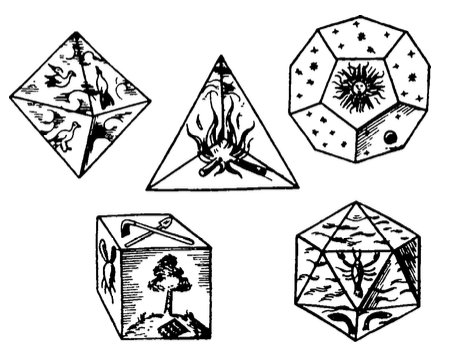
\includegraphics[width=10cm]{images/polyeder/platonic_solids.png}
\caption{Zeichnung der Platonischen Körper von Johannes Kepler aus \cite{cromwell_polyhedra_1997}. Obere Reihe (v.l.n.r.): \textit{Oktaeder}, \textit{Tetraeder}, \textit{Dodekaeder}. Untere Reihe (v.l.n.r.): \textit{Hexaeder}, \textit{Ikosaeder}.}
\label{fig:platonicsolids}
\end{figure}

\subsubsection{Polyeder}
Bevor wir die Besonderheiten der Symmetrie untersuchen, müssen wir klären, was genau ein Polyeder im mathematischen Sinne definiert. Ein Polyeder (von griechisch \textit{poly} für „viel“ und \textit{hedra} für „Sitz“ oder „Fläche“) ist ein dreidimensionaler Körper, dessen Oberfläche aus ebenen Polygonen (Vielecken) besteht. Nach Cromwell lässt sich ein Polyeder als eine Ansammlung von Flächen beschreiben, die so miteinander verbunden sind, dass sie einen abgeschlossenen Raumteil umschliessen. Dabei müssen zwei wesentliche Bedingungen erfüllt sein:

\begin{itemize}
    \item Jede Kante gehört zu genau zwei Flächen.
    \item Der Körper ist zusammenhängend: Man kann von jeder Fläche zu jeder anderen gelangen, indem man über die Kanten wandert.
\end{itemize}

Die Schnittpunkte, an denen mindestens drei Flächen (und damit mindestens drei Kanten) aufeinandertreffen, bezeichnen wir als Ecken. Ein Tetraeder besitzt beispielsweise 6 Kanten und 4 Ecken (siehe Abbildung \ref{fig:tetraeder}).

\begin{figure}[htp]
\centering
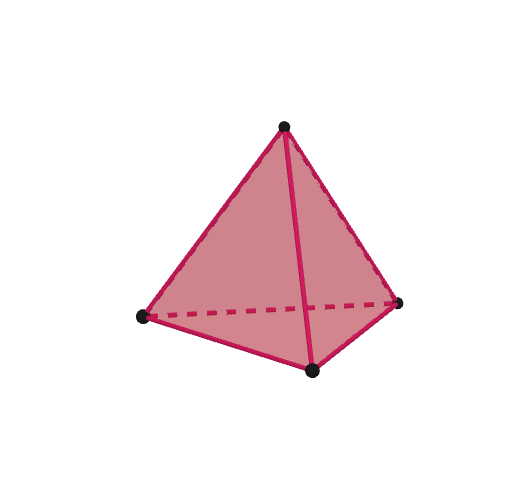
\includegraphics[width=0.4\textwidth]{images/polyeder/tetraeder.png}
\caption{Reguläres Tetraeder.}
\label{fig:tetraeder}
\end{figure}



Alltagsbeispiele für Polyeder sind etwa Pakete oder würfelförmige Regale. Sobald jedoch gekrümmte Begrenzungsflächen vorhanden sind – wie bei einer Kugel oder einer Getränkedose –, handelt es sich nicht mehr um ein Polyeder (siehe Abbildung \ref{fig:auswahl_polyeder}).

\begin{figure}[htbp]
     \centering
     \begin{subfigure}[b]{0.3\textwidth}
         \centering
         \includegraphics[width=\textwidth]{images/polyeder/kuppelhaus_düsseldorf.jpg}
         \caption{Kuppelhaus des botanischen Gartens in Düsseldorf.}
         \label{fig:kuppelhaus_düsseldorf}
     \end{subfigure}
     \hfill
     \begin{subfigure}[b]{0.3\textwidth}
         \centering
         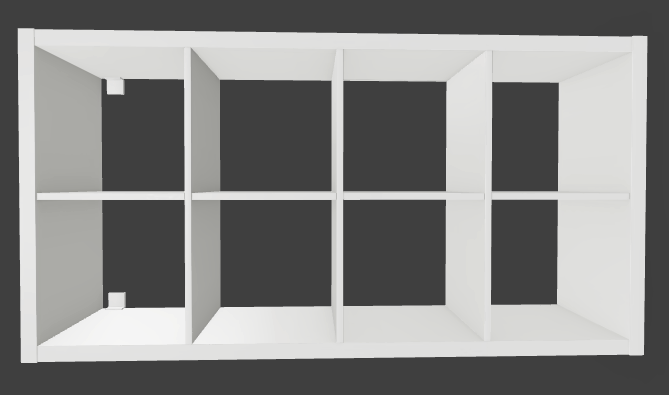
\includegraphics[width=\textwidth]{images/polyeder/kallax_ikea.png}
         \caption{Regalsystem.}
         \label{fig:kallaxikea}
     \end{subfigure}
     \hfill
     \begin{subfigure}[b]{0.3\textwidth}
         \centering
         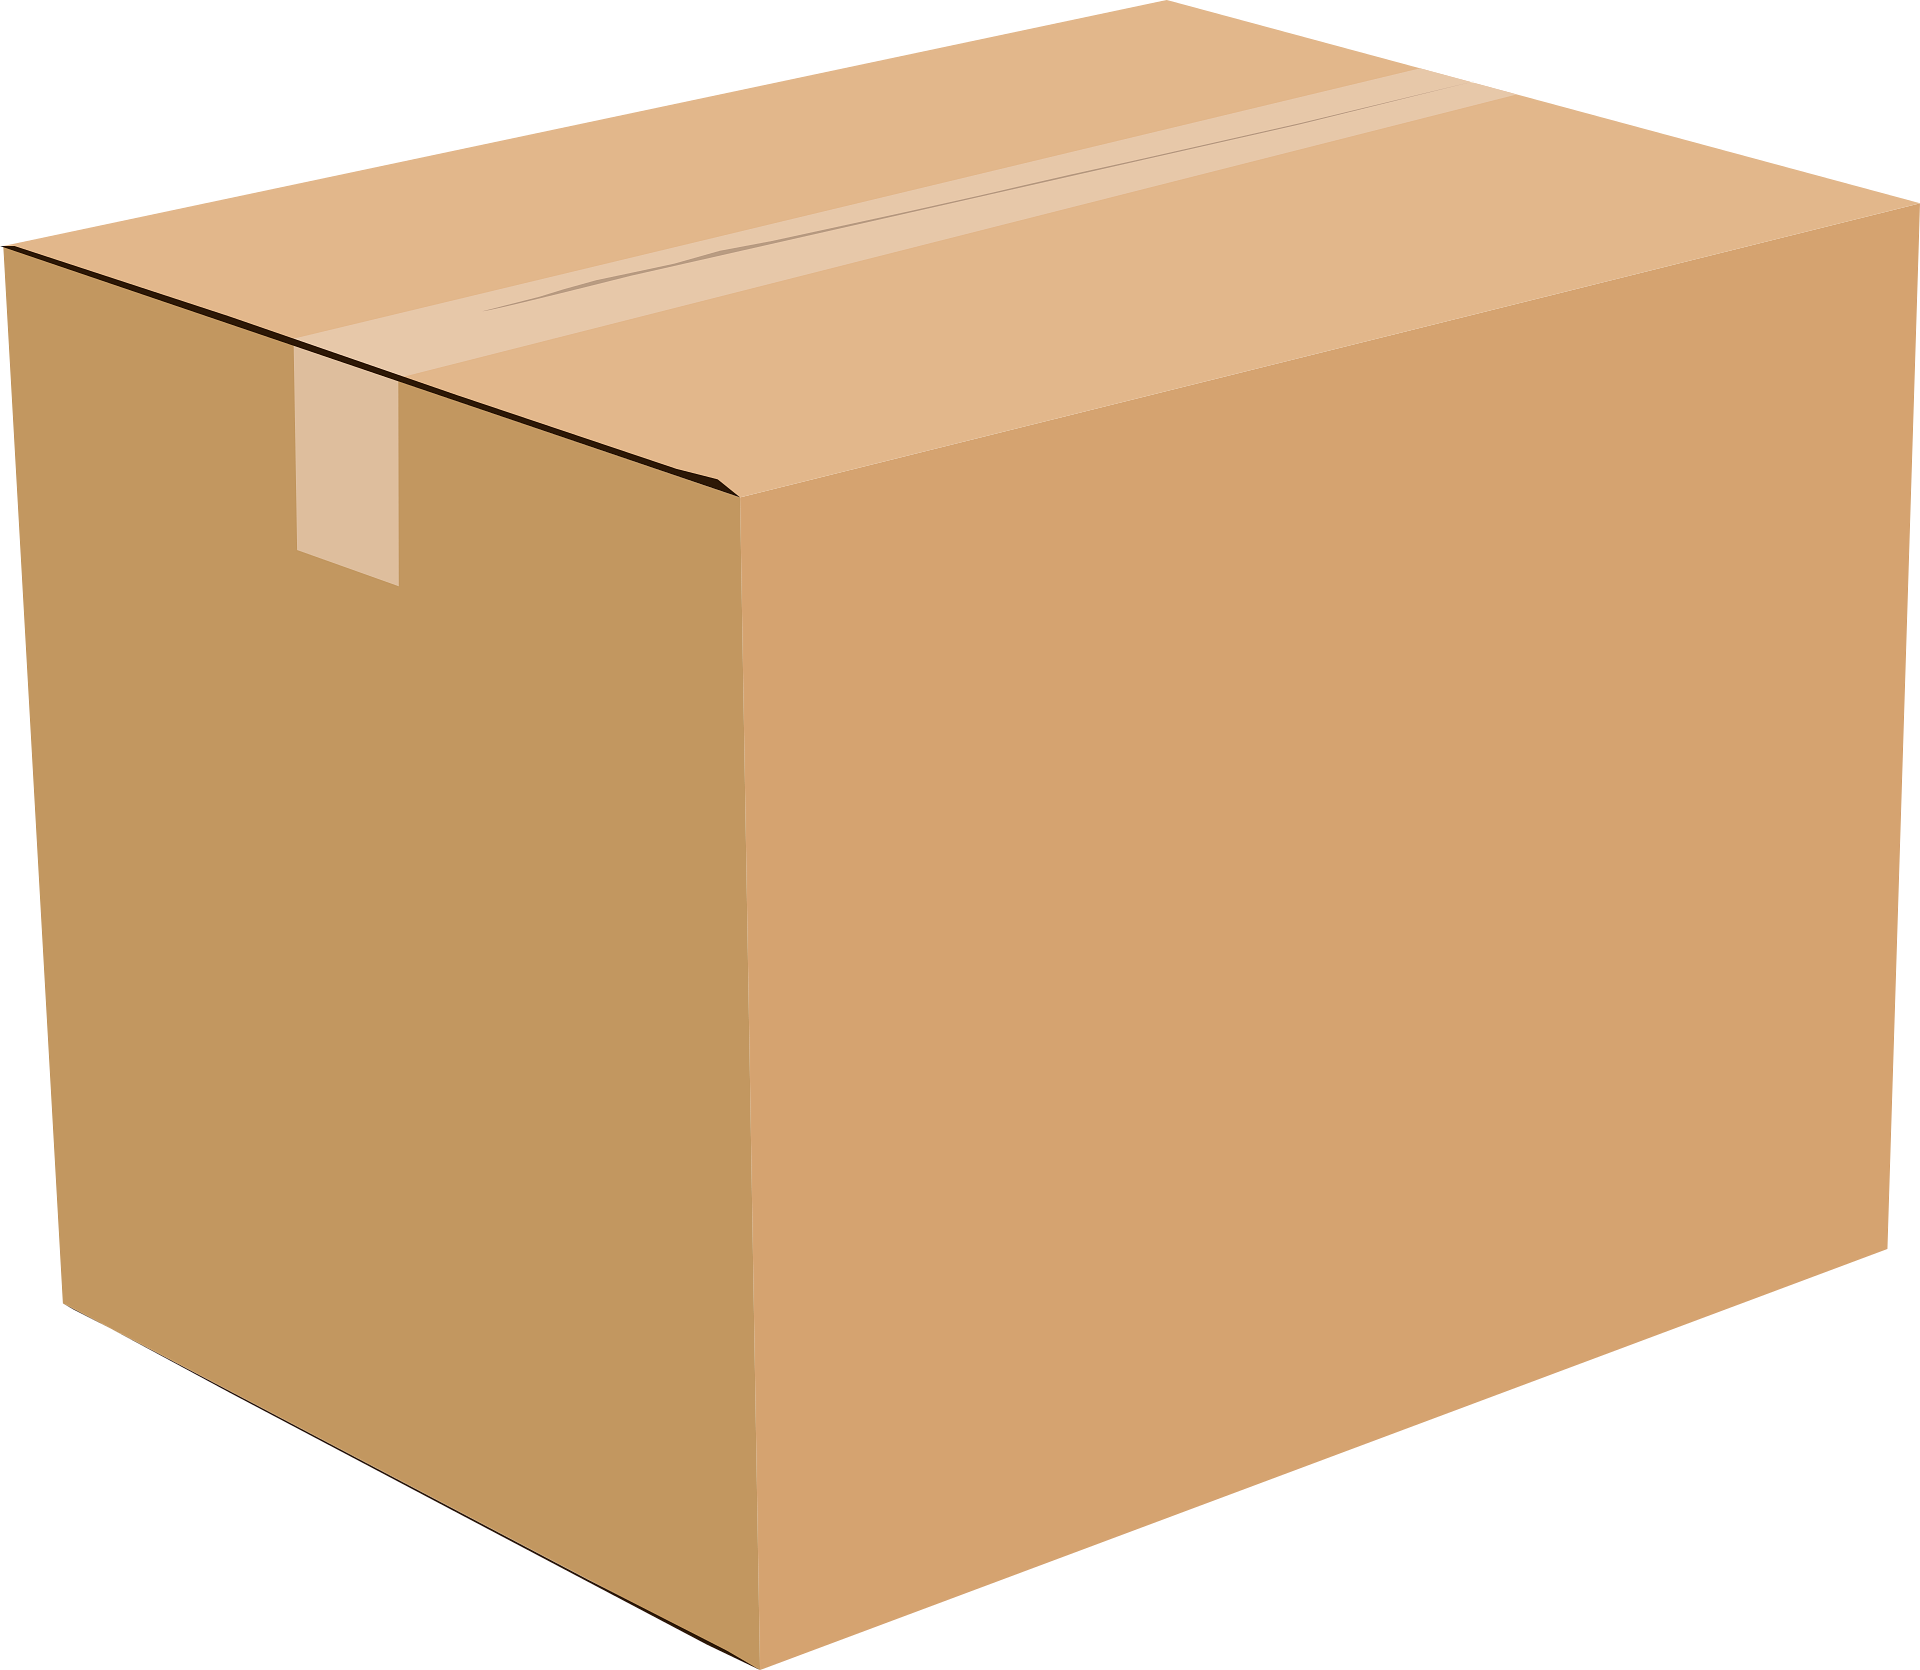
\includegraphics[width=\textwidth]{images/polyeder/paket.png}
         \caption{Quaderförmiges Paket.}
         \label{fig:Paket}
     \end{subfigure}
        \caption{Beispiele für Polyeder im Alltag und in der Architektur.}
        \label{fig:auswahl_polyeder}
\end{figure}

Damit ein Polyeder als \textit{regulär} eingestuft wird, müssen laut Coxeter zwei strenge Anforderungen an seine Regelmässigkeit erfüllt sein:

\begin{itemize}
    \item \textbf{Flächenregularität}: Alle Seitenflächen sind kongruente, reguläre Vielecke. Dies bedeutet, dass alle Kanten gleich lang und alle Innenwinkel der Flächen identisch sind.
    \item \textbf{Eckenregularität}: An jeder Ecke des Polyeders treffen stets gleich viele Flächen in der immer gleichen Anordnung zusammen.
\end{itemize}

Diese Struktur wird mathematisch durch das Schläfli-Symbol $\{p, q\}$ zusammengefasst. Dabei steht $p$ für die Anzahl der Ecken einer einzelnen Fläche und $q$ für die Anzahl der Flächen, die an einer Ecke zusammentreffen. Ein Würfel besteht aus Quadraten ($p=4$), von denen drei an jeder Ecke zusammenkommen ($q=3$), was zum Symbol $\{4, 3\}$ führt. 

Von diesen regulären Polyedern, auch als Platonische Körper bekannt, existieren exakt fünf:
\begin{itemize}
    \item \textbf{Reguläres Tetraeder}: (griech. \textit{tetra} = vier) Begrenzt von vier regulären Dreiecken.
    \item \textbf{Reguläres Hexaeder}: (griech. \textit{hex} = sechs) Der Würfel, begrenzt von sechs Quadraten.
    \item \textbf{Reguläres Oktaeder}: (griech. \textit{oktō} = acht) Begrenzt von acht regulären Dreiecken.
    \item \textbf{Reguläres Dodekaeder}: (griech. \textit{dōdeka} = zwölf) Begrenzt von zwölf regulären Fünfecken.
    \item \textbf{Reguläres Ikosaeder}: (griech. \textit{eíkosi} = zwanzig) Begrenzt von zwanzig regulären Dreiecken.
\end{itemize}



Es existieren verschiedene Beweise dafür, dass es genau fünf reguläre Polyeder gibt. Ein geometrischer Beweis von Euklid basiert auf den Innenwinkeln der Flächen. Ein weiterer, algebraischer Beweis stammt von Leonhard Euler; dieser nutzt den Polyedersatz und benötigt keine Betrachtung der Winkel. Da diese Beweise für den weiteren Verlauf dieser Arbeit nicht unmittelbar relevant sind, verweisen wir auf die entsprechende Literatur \cite[Kap.~2]{coxeter_regular_polytopes_1973, cromwell_polyhedra_1997}. Im nächsten Abschnitt werden wir uns intensiv mit den Symmetriegruppen dieser Körper beschäftigen.


\subsubsection{Aufgaben}

\begin{exercise} \label{ex:polyederalltag}
    Nennen Sie drei weitere Beispiele für Polyeder aus Ihrem Alltag, die noch nicht im Text erwähnt wurden. Begründen Sie kurz anhand der Definition, warum es sich um Polyeder handelt.
\end{exercise}

\begin{exercise} \label{ex:polyederbeispiele}
    Prüfen Sie anhand der Definition eines Polyeders, ob es sich bei den folgenden Objekten um ein solches handelt:
    \begin{itemize}
        \item[a)] der \textit{Adidas Fevernova} (offizieller Fussball der WM 2002),
        \item[b)] ein klassischer Spielwürfel mit abgerundeten Ecken.
    \end{itemize}
    Begründen Sie Ihre Antwort. Handelt es sich zudem um \textbf{reguläre} Polyeder?
\end{exercise}
\newpage
\subsection{Symmetriegruppen} \label{sec:symmetrieeigenschaftwürfel}

Wir definieren die Symmetriegruppe von einem Polyeder wie folgt
\begin{definition}
Sei $X \subset \mathbb{R}^n$ eine geometrische Figur (in unserem Fall ein Polyeder im $\mathbb{R}^3$). Eine Symmetrie von $X$ ist eine abstandserhaltende Abbildung (Isometrie) $f: \mathbb{R}^n \to \mathbb{R}^n$, die die Figur als Ganzes auf sich selbst abbildet, für die also gilt: $f(X) = X$. Die Symmetriegruppe $S(X)$ ist die Menge all dieser Symmetrien von $X$. Die Gruppenoperation ist dabei die einfache Hintereinanderausführung (Komposition) der Abbildungen.
\end{definition}

\begin{example}[Symmetriegruppe: Reguläres Tetraeder] \label{ex:regulaeres_tetraeder}
Das reguläre Tetraeder hat genau 12 Kongruenzabbildungen. Diese kann man auf mehrere Arten finden. Einerseits wissen wir, dass ein Tetraeder 6 Kanten besitzt, welche in 2 Richtungen orientiert werden können. Daraus folgt, dass es $12$ Abbildungen gibt. Andererseits können wir die Abbildungen auch zählen. 
\begin{center}
\begin{tabular}{ |c|c|c|c| } 
 \hline
 Beschreibung & Symmetrieachse & Periodizität & Anzahl Abbildungen \\ 
 \hline
 Identität & - & - & 1 \\ 
 Ecke, Mitte geg. Dreiecksfläche& K-M & $\frac{\pi}{3}$ & $2*4 = 8$  \\ 
 Kante, Kante& K-K & $\frac{\pi}{2}$ & $1*3=3$  \\ 
 \hline
  & & & 12 \\ 
 \hline
\end{tabular}
\end{center}
\end{example}

\begin{example}[Reguläres Hexaeder] \label{ex:regulaeres_hexaeder}
TODO:...
\end{example}

\begin{example}[Reguläres Ikosaeder] \label{ex:regulaeres_ikosaeder}
TODO:...
\end{example}


\subsubsection{Richtungserhaltende Abbildungen}
\begin{align}
    todo:
\end{align}


\subsubsection{Irreduzibilität}
In diesem Abschnitt untersuchen wir eine grundlegende Eigenschaft der orientierungserhaltenden Symmetriegruppen des regulären Tetraeders, Hexaeders und Ikosaeders. Wir bezeichnen mit $T$ die Gruppe der orientierungserhaltenden Symmetrien (Drehgruppe) des Tetraeders sowie analog mit $H$ und $I$ jene des Hexaeders respektive des Ikosaeders.

\begin{definition}
Sei $V$ ein Vektorraum (in unserem Fall der $\mathbb{R}^3$) und $G$ eine Gruppe von linearen Abbildungen, die auf $V$ operiert. Ein Unterraum $U \subseteq V$ heißt $G$-invariant (oder stabil unter $G$), wenn für jedes Element $g \in G$ und jeden Vektor $u \in U$ gilt, dass das Bild $g(u)$ wieder in $U$ liegt. Die Operation der Gruppe $G$ auf dem Raum $V$ heißt irreduzibel, wenn die einzigen $G$-invarianten Unterräume der triviale Nullraum $\{0\}$ und der gesamte Raum $V$ selbst sind. Gibt es hingegen einen echten invarianten Unterraum (also $U \neq \{0\}$ und $U \neq V$), so nennt man die Gruppe reduzibel.
\end{definition}


\begin{lemma} \label{lemma:irreduzibelsymmetriegruppen}
    Die orientierungserhaltenden Symmetriegruppen des Tetraeders ($T$), Hexaeders ($H$) und Ikosaeders ($I$) operieren irreduzibel auf dem $\mathbb{R}^3$. Das bedeutet, dass unter der Wirkung dieser Gruppen keine nicht-trivialen invarianten Unterräume existieren.
\end{lemma}

\begin{proof}
    Angenommen, eine Gruppe $\Omega \in \{T, H, I\}$ operiere reduzibel auf dem $\mathbb{R}^3$. Dann existiert per Definition ein echter invarianter Unterraum $U \subset \mathbb{R}^3$ der Dimension 1 (eine Gerade durch den Ursprung) oder der Dimension 2 (eine Ebene durch den Ursprung). Invariant bedeutet, dass für jedes $R \in \Omega$ und jeden Vektor $\vec{u} \in U$ auch das Bild $R\vec{u}$ wieder in $U$ liegt.

    Wir zeigen zunächst, dass in beiden Fällen eine invariante Gerade $g$ existieren muss:
    \begin{itemize}
        \item Falls $\dim(U) = 1$, ist $U$ selbst die invariante Gerade $g$.
        \item Falls $\dim(U) = 2$, muss der Normalenvektor $\vec{n}_U$ der Ebene $U$ invariant unter allen Drehungen $R \in \Omega$ sein (bis auf das Vorzeichen), da die Drehung einer Ebene deren Normale festlässt oder spiegelt. Somit bildet die durch $\vec{n}_U$ aufgespannte Gerade die gesuchte invariante Gerade $g$.
    \end{itemize}

    Sei $\vec{v}_g$ ein Richtungsvektor der Geraden $g$. Da $g$ invariant unter allen Drehungen $R \in \Omega$ ist, gibt es für das Bild $R\vec{v}_g$ nur zwei Möglichkeiten:
    \begin{itemize}
        \item $R\vec{v}_g = \vec{v}_g$ (der Vektor bleibt fix), oder
        \item $R\vec{v}_g = -\vec{v}_g$ (der Vektor wird um $180^\circ$ gedreht).
    \end{itemize}

    Nun enthalten alle betrachteten Gruppen $\{T, H, I\}$ jedoch Drehungen um $120^\circ$ (entsprechend der Symmetrie der Flächen oder Ecken). Eine $120^\circ$-Drehung kann einen Vektor nur dann auf $\vec{v}_g$ oder $-\vec{v}_g$ abbilden, wenn $\vec{v}_g$ selbst auf der Drehachse liegt. Damit die Gerade $g$ für die \textit{gesamte} Gruppe invariant ist, müsste sie also die gemeinsame Drehachse \textit{aller} $120^\circ$-Drehungen der Gruppe sein.

    Wir wissen jedoch:
    \begin{itemize}
        \item Das Tetraeder besitzt 4 solcher Drehachsen (durch die Ecken),
        \item das Hexaeder besitzt ebenfalls 4 (die Raumdiagonalen),
        \item das Ikosaeder besitzt 10 solcher Drehachsen (durch die gegenüberliegenden Ecken).
    \begin{figure}[htp]
        \centering
        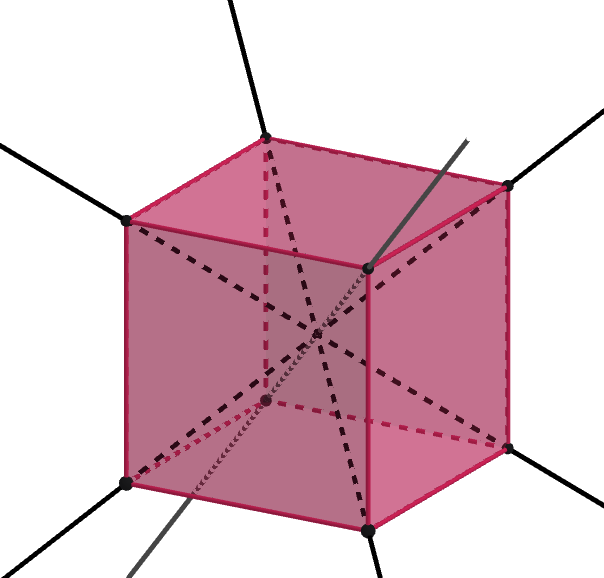
\includegraphics[width=0.6\textwidth]{images/polyeder/raumdiagonalen.png}
        \caption{Drehachsen eines regulären Hexaeders durch gegenüberliegende Ecken ($120^\circ$-Drehungen).}
        \label{fig:drehachsen}
    \end{figure}
    \end{itemize}
    Da diese Achsen nicht identisch sind, kann keine einzelne Gerade unter allen Elementen von $\Omega$ invariant sein. Dies führt zu einem Widerspruch, womit die Irreduzibilität bewiesen ist.
\end{proof}


\subsubsection{Orthogonale Matrizen} \label{sec:orthogonalrotation}
In diesem Abschnitt zeigen wir, dass Matrizen, die eine Drehung im euklidischen Raum beschreiben, stets orthogonale Matrizen sind.

\begin{lemma} \label{lemma:drehungensindorthogonalmatrizen}
    Eine Matrix $R \in \mathbb{R}^{n \times n}$, die eine Drehung repräsentiert, ist eine orthogonale Matrix. Es gilt somit $R^T R = I$, wobei $I$ die Einheitsmatrix bezeichnet.
\end{lemma}

\begin{proof}
    Seien $\vec{v}, \vec{w} \in \mathbb{R}^n$. Eine Drehung ist eine Isometrie; per Definition bleiben unter dieser Transformation zwei Eigenschaften invariant:
\begin{itemize}
    \item Die Längen der Vektoren verändern sich nicht ($\|\vec{v}\| = \|R\vec{v}\|$).
    \item Der Winkel zwischen zwei Vektoren bleibt erhalten.
\end{itemize}
Da eine Drehung somit das Skalarprodukt (und damit Längen und Winkel) erhält, muss für beliebige Vektoren $\vec{v}$ und $\vec{w}$ gelten
\begin{align*}
    (R\vec{v}) \cdot (R\vec{w}) = \vec{v} \cdot \vec{w}.
\end{align*}
Unter Verwendung der Matrixschreibweise für das Skalarprodukt $(\vec{a} \cdot \vec{b} = \vec{a}^T \vec{b})$ erhalten wir:
\begin{alignat*}{2}
    & (R\vec{v})^T (R\vec{w}) &&= \vec{v}^T\vec{w} \\
    \iff & \vec{v}^T R^T R \vec{w} &&= \vec{v}^T\vec{w} \\
    \iff & \vec{v}^T (R^T R) \vec{w} &&= \vec{v}^T I \vec{w}.
\end{alignat*}
Da diese Gleichung für alle Vektoren $\vec{v}, \vec{w} \in \mathbb{R}^n$ erfüllt sein muss, folgt daraus unmittelbar die Matrizengleichung:
\begin{align}
    R^T R = I. \nonumber
\end{align}
\end{proof}


\newpage

\subsection{Orthogonalprojektion auf eine Ebene im \texorpdfstring{$\mathbb{R}^3$}{R³}}

In diesem Text arbeiten wir primär mit Projektionen im dreidimensionalen euklidischen Raum.

\begin{definition} \label{def:orthogonalprojektion}
Sei $E \subset \mathbb{R}^3$ eine Ebene durch den Ursprung mit dem Einheitsnormalenvektor $\vec{n}$. Die Orthogonalprojektion $\Pi_E: \mathbb{R}^3 \rightarrow E$ ist eine lineare Abbildung, die jedem Vektor $\vec{v} \in \mathbb{R}^3$ seinen Bildpunkt in $E$ so zuordnet, dass der Differenzvektor $\vec{v} - \Pi_E(\vec{v})$ parallel zu $\vec{n}$ steht.
\end{definition}

Für die Beweise in Kapitel \ref{sec:orthogonalprojektionen} werden wir explizite Orthogonalprojektionen berechnen. Zur Vorbereitung leiten wir hier die allgemeine Abbildungsvorschrift her. Jeder Vektor $\vec{v}$ lässt sich eindeutig in zwei Komponenten zerlegen:
\begin{align} \label{eq:vektor_parallel_senkrecht}
    \vec{v} = \vec{v}_{\parallel} + \vec{v}_{\perp},
\end{align}
wobei gilt:
\begin{itemize}
    \item $\vec{v}_{\parallel}$ liegt in der Ebene $E$ (die projizierte Komponente),
    \item $\vec{v}_{\perp}$ steht senkrecht auf der Ebene $E$ und ist somit parallel zum Einheitsnormalenvektor $\vec{n}$.
\end{itemize}

Da $\vec{v}_{\perp}$ parallel zu $\vec{n}$ ist, existiert ein Skalar $\alpha \in \mathbb{R}$ mit $\vec{v}_{\perp} = \alpha \vec{n}$. Um $\alpha$ zu bestimmen, bilden wir das Skalarprodukt mit $\vec{n}$:
\begin{align} \label{eq:skalar_senkrecht}
    \vec{n} \cdot \vec{v} &= \vec{n} \cdot (\vec{v}_{\parallel} + \vec{v}_{\perp}) \nonumber \\
    &= \vec{n} \cdot \vec{v}_{\parallel} + \vec{n} \cdot (\alpha \vec{n}) \nonumber \\
    &= 0 + \alpha (\vec{n} \cdot \vec{n}) = \alpha,
\end{align}
wobei wir $\vec{n} \cdot \vec{v}_{\parallel} = 0$ (da $\vec{v}_{\parallel} \in E$) und $\vec{n} \cdot \vec{n} = 1$ (da $\|\vec{n}\|=1$) genutzt haben. Einsetzen in \eqref{eq:vektor_parallel_senkrecht} liefert:

\begin{align} \label{eq:projectionwithvectorandnormal}
    \Pi_{E}(\vec{v}) &= \vec{v}_{\parallel} = \vec{v} - \vec{v}_{\perp} \nonumber \\
    &= \vec{v} - \alpha \vec{n} \nonumber \\
    &= \vec{v} - (\vec{n} \cdot \vec{v}) \vec{n}.
\end{align}



In Matrixschreibweise lässt sich das Skalarprodukt $(\vec{n} \cdot \vec{v})\vec{n}$ als dyadisches Produkt $\vec{n}\vec{n}^T \vec{v}$ ausdrücken. Damit erhalten wir die Projektionsmatrix:

\begin{align} \label{eq:ortho_proj_matrix_notation}
    \Pi_{E}(\vec{v}) &= \vec{v} - (\vec{n}\vec{n}^T) \vec{v} \nonumber \\
    &= (I - \vec{n}\vec{n}^T) \vec{v}.
\end{align}

\subsubsection{Aufgaben}
\begin{exercise} \label{ex:verifizierungwuerfelprojektion}
Verifizieren Sie die Resultate für die Ebenen $E_1$ und $E_2$ aus Beispiel \ref{ex:wuerfelprojektionen} mithilfe der Matrixdarstellung aus Gleichung \eqref{eq:ortho_proj_matrix_notation}.
\end{exercise}


\section{Invarianz der Orthogonalprojektion} \label{sec:orthogonalprojektionen}
In diesem Kapitel untersuchen wir die Orthogonalprojektionen von Polyedern mit spezifischen Symmetrieeigenschaften auf beliebige Ebenen im Raum. Wir folgen dabei der Argumentation von Hungerbühler und Zhang \cite{hungerbuehler_symmetric_polyhedra}.

\subsection{Symmetrische Polyeder und Kantenprojektionen}
Wie bereits im Einführungsbeispiel (siehe Beispiel \ref{ex:wuerfelprojektionen_revisited} und Aufgabe \ref{ex:verifizierungwuerfelprojektion}) aufgezeigt wurde, ist die Summe der quadrierten Längen der projizierten Kanten eines regulären Hexaeders unter einer Orthogonalprojektion unabhängig von der gewählten Projektionsebene. Diese Invarianzeigenschaft lässt sich jedoch nicht nur beim regulären Hexaeder beobachten, sondern allgemein bei Polyedern, deren Symmetrie.

\begin{theorem} \label{satz:sum_projection_independent_of_plane}
    Sei $P \subset \mathbb{R}^3$ ein Polyeder, dessen Symmetriegruppe eine der Gruppen $T$, $H$ oder $I$. Sei ferner $\Pi_{E}: \mathbb{R}^3 \to E$ die Orthogonalprojektion auf eine Ebene $E \subset \mathbb{R}^3$. Dann ist die Summe der Quadrate der projizierten Kantenlängen von $P$ unabhängig von der Wahl der Ebene $E$, das heisst:
    \begin{align} \label{eq:sum_projection_independent_of_plane}
        \sum_{k \in K_{P}} \|\Pi_{E_1}(\vec{v}_k)\|^2 = \sum_{k \in K_P} \|\Pi_{E_2}(\vec{v}_k))\|^2,
    \end{align}
    wobei $K_{P}$ die Menge der Kanten von $P$ bezeichnet und $\vec{v}_k)$ der Richtungsvektor der Kante $k$ ist.
\end{theorem}

Um ein tieferes Verständnis für Satz \ref{satz:sum_projection_independent_of_plane} und dessen geometrische Konsequenzen zu gewinnen, betrachten wir im Folgenden erneut die Ergebnisse aus Aufgabe \ref{ex:verifizierungwuerfelprojektion} unter diesem neuen theoretischen Gesichtspunkt.

\begin{example}
    Wir erinnern uns an unser Einstiegsbeispiel, bei dem wir für die Summe der quadrierten projizierten Kantenlängen den folgenden Wert erhalten haben:
    \begin{align} \label{eq:summewürfelorthogonalprojektion_second_revisit}
        \sum_{\vec{v}_k \in K_W} \|\Pi_{E_1}(\vec{v}_k)\|^2 = 8.
    \end{align}
    Dabei bezeichnet $K_W$ die Menge der Kanten des regulären Hexaeders $W$ und $E_1$ die Ebene $$x+y+z=0.$$ 
    
    Gemäss Satz \ref{satz:sum_projection_independent_of_plane} ist dieser Wert unabhängig von der Wahl der Ebene. Das bedeutet: Unabhängig davon, auf welche Ebene $E \subset \mathbb{R}^3$ wir die Würfelkanten projizieren, die Summe der Quadrate wird stets $8$ ergeben. Es ist jedoch zu beachten, dass dieser spezifische Wert $8$ an die Kantenlänge des Einheitswürfels gebunden ist. Bei einem skalierten Hexaeder bleibt die Summe zwar ebenfalls invariant gegenüber der Wahl der Ebene, der konstante Wert weicht jedoch von $8$ ab. Dies beendet unser Beispiel.
\end{example}

Bevor wir Satz \ref{satz:sum_projection_independent_of_plane} allgemein beweisen, skizzieren wir die grundlegende Beweisidee. Sei $P \subset \mathbb{R}^3$ ein Polyeder mit der Symmetriegruppe $\Omega \in \{T, H, I\}$. Mithilfe von $\Omega$ lassen sich die Kanten von $P$ in Äquivalenzklassen (Bahnen) unterteilen. Zwei Kanten $k_1, k_2$ sind äquivalent, wenn sie durch ein Element der Symmetriegruppe ineinander überführt werden können:
\begin{align}
    k_1 \sim k_2 :\iff \exists w \in \Omega: w(k_1) = k_2. \nonumber
\end{align}
Da die Menge der Kanten $K_P$ die disjunkte Vereinigung dieser Äquivalenzklassen ist, reicht es aus, die Aussage des Satzes für alle einzelnen Klassen zu zeigen. Wir müssen also nachweisen, dass die Summe der quadrierten Projektionslängen für alle Kanten innerhalb einer solchen Symmetrie-Bahn invariant gegenüber der Wahl der Ebene ist.


% Proof of lemma 1
\begin{lemma} \label{lemma:quadriertesummeinvarianzstrecken}
    Sei $s \subset \mathbb{R}^3$ eine Strecke, $\Omega$ einer der Symmetriegruppen $T$, $H$, $I$ und $\Pi_{E}:\mathbb{R}^3 \rightarrow E$ die orthogonale Projektion auf eine Ebene $E \subset \mathbb{R}^3$. Dann ist die Summe  
    \begin{align} \label{eq:sum_line_segment_projection_independent_of_plane}
        \sum_{w \in \Omega} \|\Pi_{E}w(s)\|^2  
    \end{align}
    unabhängig von $E$.
\end{lemma}

\begin{proof} 
Wir werden den Beweis nur für $\Omega = T$ zeigen, da wir einerseits noch einen Alternativbeweis zeigen und andererseits der Beweis analog für $\Omega \in \{H,I\}$ funktioniert. Sei $\Omega = T$. Wir wollen in diesem Beweis konkret nachrechnen, dass die Summe in Gleichung \eqref{eq:sum_line_segment_projection_independent_of_plane} konstant ist. Dafür müssen wir die Projektionen ausrechnen. Für die Orthogonalprojektion $\Pi_{E}$ gilt gemäss \eqref{eq:ortho_proj_matrix_notation}
\begin{align} 
    \Pi_{E}(\vec{v}) = (I - \vec{n}\vec{n}^T) \vec{v} = I - \begin{pmatrix}
        n_1^2 & n_1 n_2 & n_1 n_3 \\
        n_2 n_1 & n_2^2 & n_2 n_3 \\
        n_3 n_1 & n_3 n_2 & n_3^2
    \end{pmatrix}. \nonumber
\end{align}
Wie wir wissen, gilt $|T|=12$. Das bedeutet, wir müssen die $12$ Abbildungen ausrechnen. Dazu betrachten wir folgendes Tetraeder mit Kanten $(1,1,1)$, $(1,-1,-1)$, $(-1,1,-1)$ und $(-1,-1,1)$, siehe Abbildung \ref{fig:tetraederspezielleorientierung}.
\begin{figure}[htp]
    \centering
    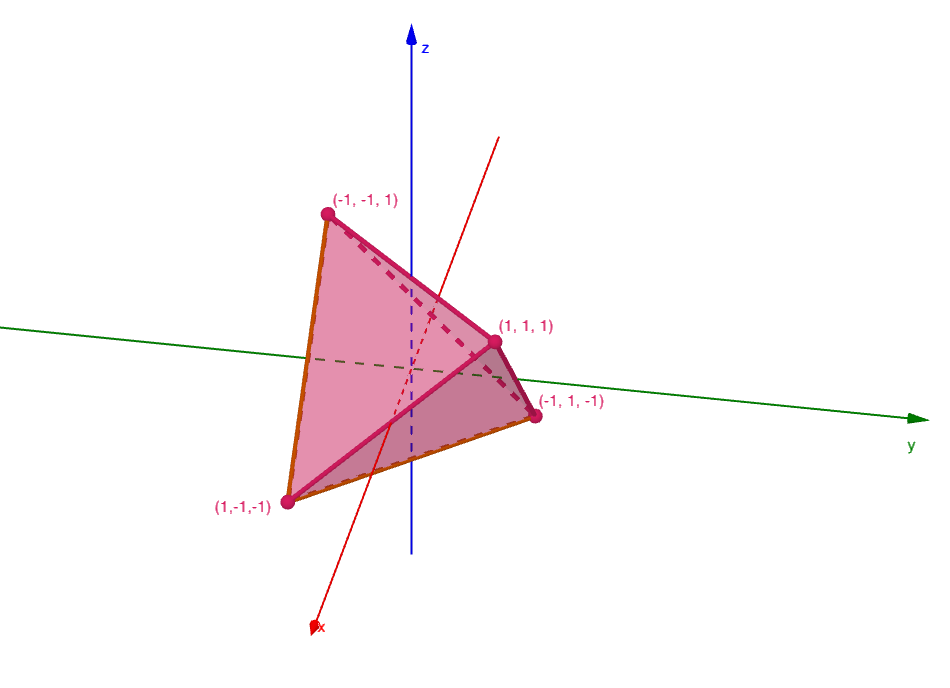
\includegraphics[width=0.6\textwidth]{images/polyeder/tetraederspeziellorientiert.png}
    \caption{Tetraeder mit Kanten $(1,1,1)$, $(1,-1,-1)$, $(-1,1,-1)$ und $(-1,-1,1)$.}
    \label{fig:tetraederspezielleorientierung}
\end{figure}
Wenn wir diese spezielle Ausrichtung des Tetraeders wählen, können wir die Rotationen um die Achsen von Typ $b$, siehe Abbildung \ref{fig:tetraederotationsachsen}, wie folgt darstellen:

\begin{align}
    A_0 = \begin{pmatrix} 1 & 0 & 0 \\ 0 & 1 & 0 \\ 0 & 0 & 1 \end{pmatrix}, \quad
    A_1 = \begin{pmatrix} 1 & 0 & 0 \\ 0 & -1 & 0 \\ 0 & 0 & -1 \end{pmatrix}, \nonumber \\
    A_2 = \begin{pmatrix} -1 & 0 & 0 \\ 0 & 1 & 0 \\ 0 & 0 & -1 \end{pmatrix}, \quad
    A_3 = \begin{pmatrix} -1 & 0 & 0 \\ 0 & -1 & 0 \\ 0 & 0 & 1 \end{pmatrix}. \nonumber
\end{align}
Die Rotation von Typ $a$ lässt sich mit der Matrix
\begin{align}
    R &= \begin{pmatrix} 0 & 0 & 1 \\ 1 & 0 & 0 \\ 0 & 1 & 0 \end{pmatrix} \nonumber
\end{align}
darstellen. Alle Abbildungen der Symmetriegruppe $T$ sind somit gegeben durch
$$ \left\{A_i R^k \mid k \in \{0,1,2\}, i \in \{0,1,2,3\} \right\}.$$
Somit können wir nun die Summe berechnen und wir erhalten
\begin{align}
    \sum_{w \in \Omega} \|\Pi_{E}w(s)\|^2  &= \sum_{k=0}^2 \sum_{i=0}^3 \|\Pi_{E}A_iR^k\|^2 \nonumber \\ 
    &=  \sum_{k=0}^2 \sum_{i=0}^3 \left\|\left(I - \begin{pmatrix}
        n_1^2 & n_1 n_2 & n_1 n_3 \\
        n_2 n_1 & n_2^2 & n_2 n_3 \\
        n_3 n_1 & n_3 n_2 & n_3^2
    \end{pmatrix}\right)A_iR^k\vec{s} \ \right\|^2  \nonumber \\
    &=8 \|\vec{s}\|^2, \nonumber
\end{align}
wobei wir die Tatsache benutzt haben, dass die Strecke $s$ unter Translation ihre Länge nicht verändert. Inbesondere, dass wir die Strecke $s$ auf den Ursprung verschieben können und dementsprechend $s$ als Vektor $\vec{s} \in \mathbb{R}^3$ betrachten können. 
\end{proof}
Wir möchten hier anmerken, dass das Ausmultiplizieren der Matrizen im Beweis keine schwierige, jedoch eine zeitintensive Aufgabe ist. Wir ermutigen die LeserInnen zumindest einmal die Rechnung selbst per Hand auszurechnen. Wie schon im Beweis erwähnt, folgen die Beweise für $\Omega \in \{H,I\}$ demselben Schema. Da die Kardinalität der Symmetriegruppen jedoch grösser ist, wird der Rechenaufwand dementsprechend auch grösser. Da kommt es gerade gelegen, dass wir anstatt die Summe der Kantenlängen unter der Orthogonalprojektion, siehe Gleichung \eqref{eq:sum_projection_independent_of_plane}, direkt auszurechnen, auch über die Irreduzibilität von den Symmetriegruppen den Beweis führen können.
\begin{proof}
    Sei $\vec{s} \in \mathbb{R}^3$ der Richtungsvektor der Strecke $s$. Wir nutzen die Zerlegung aus Gleichung \eqref{eq:vektor_parallel_senkrecht} und die Darstellung der Projektionslänge aus \eqref{eq:projectionwithvectorandnormal}. Für ein beliebiges $w \in \Omega$ gilt:
    \begin{align} 
        \|\Pi_{E}w(\vec{s})\|^2 &= \|w_{\parallel}(\vec{s})\|^2 \nonumber \\
        &= \|w(\vec{s})\|^2 - \|w(\vec{s})_{\perp}\|^2 \nonumber \\
        &= \|w(\vec{s})\|^2 - \|\left(\vec{n}_E \cdot w(\vec{s})\right)\vec{n}_E\|^2, \nonumber
    \end{align}
    wobei $\vec{n}_E$ der Normalenvektor der Ebene $E$ ist, d.h. $\|\vec{n}_E\| = 1$. Da alle Abbildungen $w \in \Omega$ Drehungen und somit Isometrien (längenerhaltend) sind, gilt $\|w(\vec{s})\|^2 = \|\vec{s}\|^2$. Summiert über die gesamte Gruppe ergibt sich:
    \begin{align} 
        \sum_{w \in \Omega} \|\Pi_{E}w(\vec{s})\|^2 &= \sum_{w \in \Omega} \left( \|w(\vec{s})\|^2 - \|\left(\vec{n}_E \cdot w(\vec{s})\right)\vec{n}_E\|^2 \right) \nonumber \\
        &= \sum_{w \in \Omega} \left( \|\vec{s}\|^2 - |\vec{n}_E \cdot w(\vec{s})|^2 \|\vec{n}_E \|^2\right) \nonumber \\
        &= |\Omega|  \|\vec{s}\|^2 - \sum_{w \in \Omega} |\vec{n}_E \cdot w(\vec{s})|^2. \nonumber
    \end{align}
    Der erste Term $|\Omega| \cdot \|\vec{s}\|^2$ ist konstant. Um die Unabhängigkeit bezüglich der Ebene $E$ zu zeigen, müssen wir nachweisen, dass auch der zweite Term konstant ist. Unter Verwendung der Identität $(\vec{a} \cdot \vec{b})^2 = \vec{a}^T(\vec{b} \ \vec{b}^T)\vec{a}$ erhalten wir:
    \begin{align} \label{eq:summevectormatrixnormal_revised}
        \sum_{w \in \Omega} |\vec{n}_E \cdot w(\vec{s})|^2 &= \sum_{w \in \Omega} \vec{n}_E^T \left( w(\vec{s}) w(\vec{s})^T \right) \vec{n}_E \nonumber \\
        &= \vec{n}_E^T \left( \sum_{w \in \Omega} w(\vec{s}) w(\vec{s})^T \right) \vec{n}_E.
    \end{align}
    Wir definieren die Matrix $$M := \sum_{w \in \Omega} w(\vec{s}) w(\vec{s})^T \in \mathbb{R}^{3 \times 3}.$$ 
        Das bedeutet, unsere Summe aus Gleichung \eqref{eq:sum_line_segment_projection_independent_of_plane} lässt sich wie folgt schreiben
       \begin{align} \label{eq:summemitmatrixM}
        \sum_{w \in \Omega} \|\Pi_{E}w(\vec{s})\|^2 = |\Omega|  \|\vec{s}\|^2 - \vec{n}_E^T M \vec{n}_E.
    \end{align}
    Nun stellt sich uns die Frage, wann der hintere Term konstant ist. Zuerst tragen wir jedoch zusammen, welche Eigenschaften die Matrix $M$ hat:
    \begin{itemize}
        \item[I.]  Die Matrix $M$ ist symmetrisch ($M=M^T$). Gemäss dem Spektralsatz, siehe Anhang \ref{sec:spektralsatzlinearealgebra}, besitzt die symmetrische Matrix $M$ einen reellen Eigenwert $\lambda$ mit zugehörigem Eigenraum $V_\lambda \neq \{0\}$.
        \item[II.] Die Matrix $M$ kommutiert mit jeder Drehung $R \in \Omega$:
    \begin{align}
        R M R^T &= \sum_{w \in \Omega} R w(\vec{s}) w(\vec{s})^T R^T = \sum_{w \in \Omega} (R w(\vec{s})) (R w(\vec{s}))^T= M, \nonumber
    \end{align}
 da die Multiplikation mit $R$ von links die Gruppenelemente lediglich permutiert. Wie wir bereits in Abschnitt \ref{sec:orthogonalrotation} gesehen haben, sind Drehungen orthogonal und es folgt 
 \begin{align} 
    RM = MR. \nonumber
 \end{align}
    \end{itemize}

 Für einen Vektor $\vec{v} \in V_\lambda$ gilt somit
    \begin{align}
        M(R\vec{v}) \overset{II.}{=} R(M\vec{v}) \overset{I.}{=} R(\lambda \vec{v}) = \lambda (R\vec{v}). \nonumber
    \end{align}
    Somit ist $R\vec{v} \in V_\lambda$, was bedeutet, dass $V_\lambda$ ein invarianter Unterraum unter der Wirkung von $\Omega$ ist. Da die Gruppen $T, H$ und $I$ nach Lemma \ref{lemma:irreduzibelsymmetriegruppen} irreduzibel auf dem $\mathbb{R}^3$ operieren, muss $V_\lambda = \mathbb{R}^3$ gelten. Daraus folgt, dass $M$ ein skalares Vielfaches der Einheitsmatrix ist: $$M = \lambda I_3.$$
    
    Eingesetzt in Gleichung \eqref{eq:summevectormatrixnormal_revised} ergibt sich:
    \begin{align}
        \sum_{w \in \Omega} |\vec{n}_E \cdot w(s)|^2 = \vec{n}_E^T (\lambda I_3) \vec{n}_E = \lambda (\vec{n}_E^T \vec{n}_E) = \lambda. \nonumber
    \end{align}
    Da $\lambda$ eine Konstante ist, ist die Summe der quadrierten Projektionslängen unabhängig von der Ebene $E$.
\end{proof}





Beachte, dass im Gegensatz zum direkten Beweis, der explizite Wert der Summe in Gleichung \eqref{eq:sum_line_segment_projection_independent_of_plane} nicht berechnet wird. Nun haben wir alles beisammen, um die Aussage in Satz \ref{satz:sum_projection_independent_of_plane} zu beweisen.

\begin{proof}
    Sei $P$ ein Polyeder mit Symmetriegruppe $\Omega = T, H$ oder $I$. TODO:...
\end{proof}

Beachte, dass der Tetraeder, Hexaeder und Ikosaeder alle nur eine Äquivalenzklasse haben. Um ein Objekt zu finden, welches eines der Symmetriegruppen $T$, $H$ oder $I$ hat und mehrere Äquivalenzklassen aufweist, braucht es etwas kreativität. Ein Beispiel ist das Chiral-Polyeder in Abbildung \ref{fig:chiralpolyeder}.
\begin{figure}[htp]
    \centering
    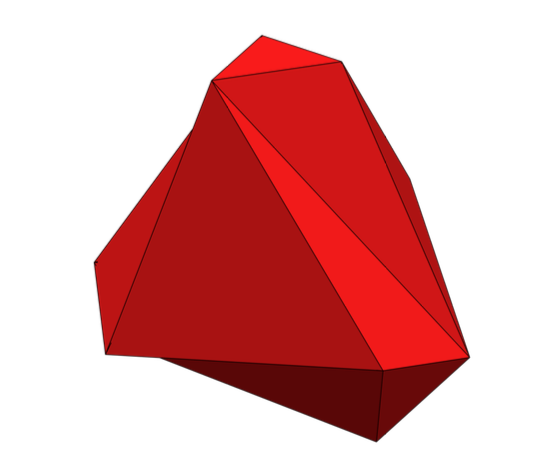
\includegraphics[width=10cm]{images/polyeder/chiral_polyeder.png}
    \caption{Ein Chiral-Polyeder mit Symmetriegruppe $T$, welches mehrere Äquivalenzklassen aufweist.\protect\footnotemark}
    \label{fig:chiralpolyeder}
\end{figure}
\footnotetext{Quelle: \cite{hungerbuehler_symmetric_polyhedra}}

\begin{example} \label{example:geradesprisma}
    Eine Frage, die man sich stellen könnte, ist, wieso der Beweis für Lemma \ref{lemma:quadriertesummeinvarianzstrecken} nicht für andere Symmetriegruppen funktioniert. Dafür betrachten wir zum Beispiel ein gerades Prisma mit einem $n$-Eck als Grunfläche, siehe Abbildung \ref{fig:geradesprisma}. 
    \begin{figure}[htp]
    \centering
    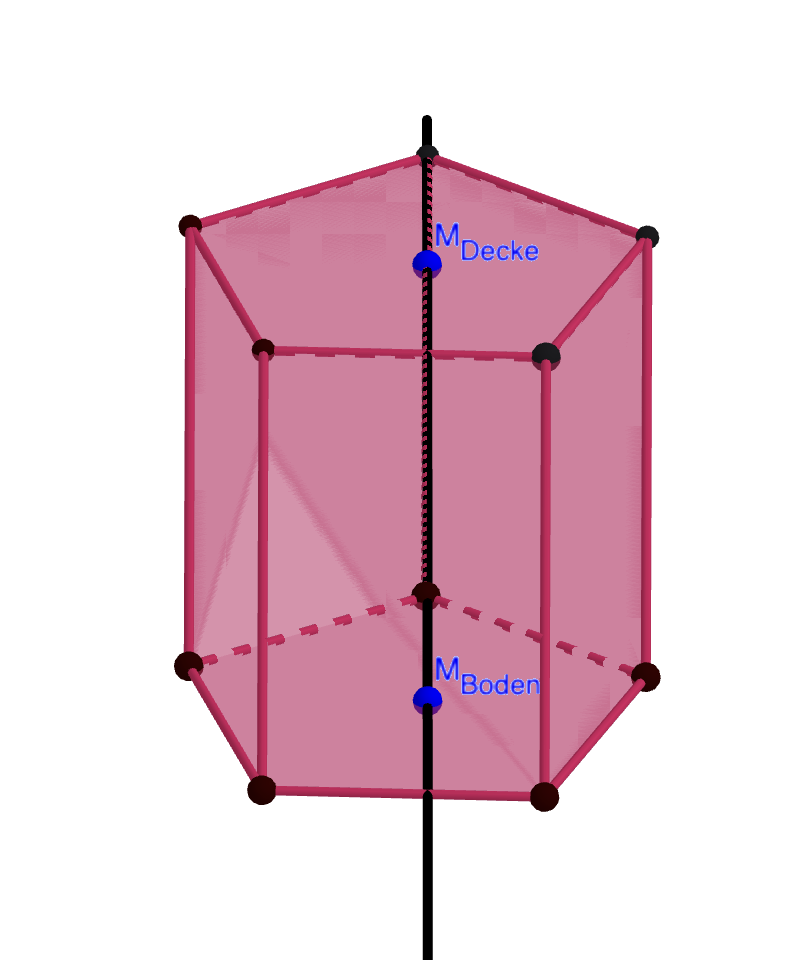
\includegraphics[width=0.4\textwidth]{images/prisma_z_achse.png}
    \caption{Gerades Prisma mit einem $5$-Eck als Grundfläche.}
    \label{fig:geradesprisma}
\end{figure}
    Die Symmetriegruppe vom geraden Prisma ist die \textit{Diedergruppe $D_n$}, welches die Symmetriegruppe des regulären $n$-Ecks ist. Die orientierungserhaltenden Kongruenztransformationen sind die Drehungen, um die Achse, welche durch die Mittelpunkte, $M_{\text{Boden}}$ und $M_{\text{Decke}}$ der $5$-Ecke verläuft (Sowie der achse durch eine Kante und mittelpunkt). Somit ist die z-Achse ein nicht-trivialer invarianter Unterraum $U \subset \mathbb{R}^3$ und folglich $D_n$ nicht irreduzibel. Somit würde der Beweis nicht mehr funktionieren. Stattdessen berechnen wir zuerst einmal die Matrix $M:= \sum_{w \in \Omega} w(\vec{s}) w(\vec{s})^T$. Beachte, dass wir in diesem Fall zwei Orbits haben: Die Höhenkanten sowie die Kanten vom $n-$Eck, am Boden sowie an der Decke. Das heisst für die Matrix $M$ gilt
    \begin{align}
        M = M_{\text{Höhenkanten}} + M_{\text{Kanten n-Eck}}. \nonumber
    \end{align}
    Für die Höhenkanten gilt 
    \begin{align}
        M_{\text{Höhenkanten}}=& \sum_{w \in D_n} \begin{pmatrix} 0 \\ 0 \\ h \end{pmatrix} \begin{pmatrix} 0 \\ 0 \\ h \end{pmatrix}^T \nonumber \\
        =& \begin{pmatrix} 0 & 0 & 0 \\ 0 & 0 & 0 \\ 0 & 0 & n  h^2 \end{pmatrix}. \nonumber 
    \end{align}
    Analog gilt
    \begin{align}
        M_{\text{Kanten n-Eck}} &= \sum_{w \in D_n}\begin{pmatrix} x_i \\ y_i \\ 0 \end{pmatrix} \begin{pmatrix} x_i & y_i & 0 \end{pmatrix} \nonumber \\
        &= n\begin{pmatrix} x_i^2 & x_i y_i & 0 \\ x_i y_i & y_i^2 & 0 \\ 0 & 0 & 0 \end{pmatrix} \nonumber \\
        &= \begin{pmatrix} n  a^2 & 0 & 0 \\ 0 & n  a^2 & 0 \\ 0 & 0 & 0 \end{pmatrix}. \nonumber
    \end{align}
    Es folgt
    \begin{align}
        M = \begin{pmatrix} n  a^2 & 0 & 0 \\ 0 & n  a^2 & 0 \\ 0 & 0 & nh^2 \end{pmatrix}. \nonumber
    \end{align}
    Daraus folgen zwei Fälle
    \begin{itemize}
        \item Fall $a \neq h$: $M \neq \lambda I_3 \implies $ Die Summe der quadrierten Kantenlängen unter eine Orthogonalprojektion sind nicht unabhängig von der Ebene.
        \item Fall $a = h$: $M = na^2 I_3 \implies $ Die Summe \eqref{eq:sum_line_segment_projection_independent_of_plane} bleibt, unabhängig von der Ebene, konstant.
    \end{itemize}
    Dies beendet unser Beispiel.
\end{example}


Eine interessante Beobachtung von Beispiel \ref{example:geradesprisma} ist, dass die Bedingungen in Satz (\ref{satz:sum_projection_independent_of_plane}) eine hinreichende, aber keine notwendige Bedingung ist für die Projektionseigenschaft (siehe Gleichung (\ref{eq:sum_projection_independent_of_plane})). Das heisst es existieren Polyeder, welche die Projektionseigenschaft erfüllen, aber nicht die Symmetrieeigenschaften besitzen. Ein Beispiel dafür ist das gerade Prisma mit $a=h$. Ein weiteres Beispiel ist der Pseudo-Rhombenkuboktaeder, siehe Abbildung \ref{fig:Pseudorhombicuboctahedron}. \footnote{Nicht zu verwechseln mit dem Rhombenkuboktaeder (siehe Abschnitt \ref{sec:rhombenkuboktaeder}).}

\begin{figure}[htp]
    \centering
    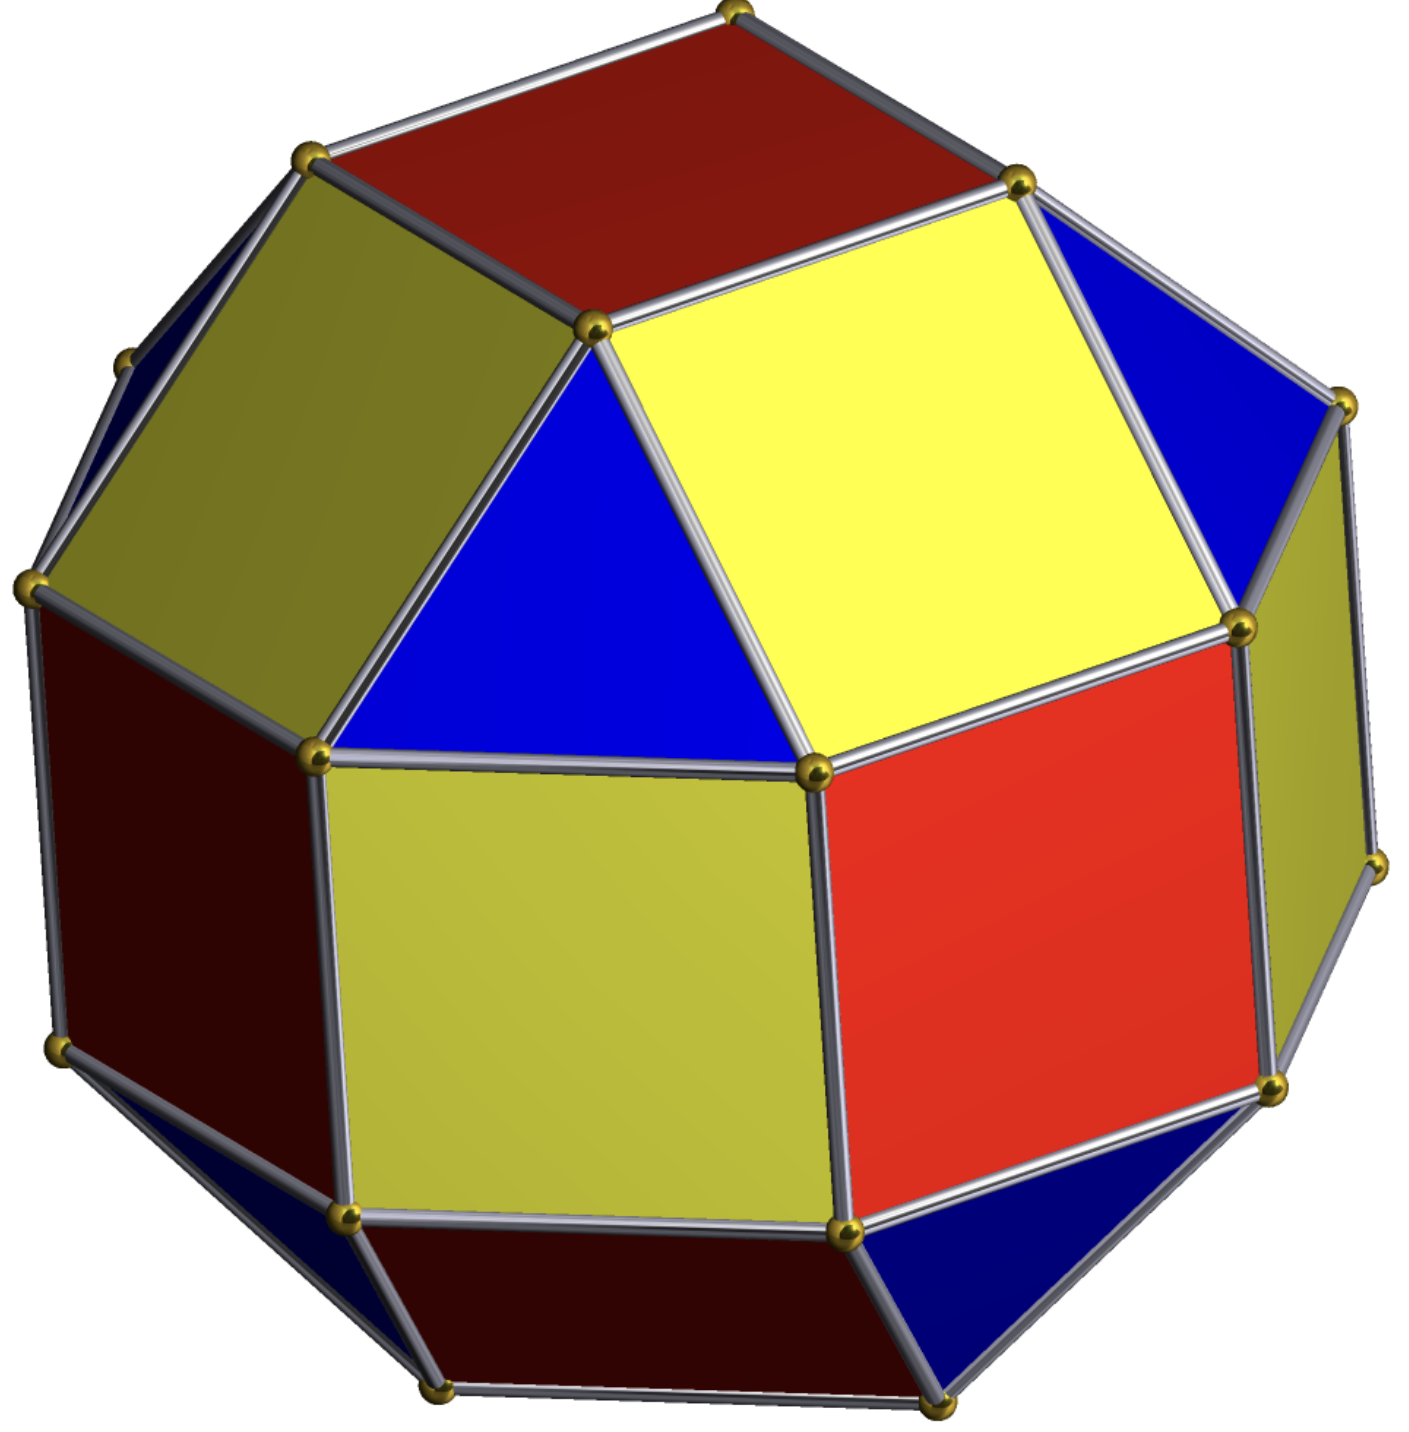
\includegraphics[width=10cm]{images/polyeder/Pseudorhombicuboctahedron.png}
    \caption{Pseudo-Rhombenkuboktaeder (elongated square gyrobicupola), Wikipedia \cite{elongated_square_gyrobicupola}.}
    \label{fig:Pseudorhombicuboctahedron}
\end{figure}
\begin{example} [Symmetriegruppe Pseudo-Rhombenkuboktaeder]
    Eine unserer Behauptungen ist, dass der Pseudo-Rhombenkuboktaeder keine der Symmetriegruppen T, H oder I hat. Wenn wir das Pseudo-Rhombenkuboktaeder (siehe Abbildung \ref{fig:Pseudorhombicuboctahedron}) betrachten, stellen wir fest, dass wir eine Symmetrieachse 4.\ Orndung haben. Diese geht vertikal durch das obere und untere rote Quadrat ("Deckel" und "Boden"). Da die Symmetriegruppe T gar keine Symmetrieachse 4.\ Ordnung hat, können wir ausschliessen, dass der Pseudo-Rhombenkuboktaeder die Symmetriegruppe T hat. Bemerke, dass das Pseudo-Rhombenkuboktaeder genau eine Symmetrieachse 4.\ Ordnung besitzt. Analog können wir auch die Symmetriegruppen H und I ausschliessen (siehe Aufgaben \ref{ex:PseudoRhombenkuboktaeder_Symmetriegruppe}).
\end{example}

Es bleibt also noch zu zeigen, dass das Pseudo-Rhombenkuboktaeder die Gleichung 
(\ref{eq:sum_projection_independent_of_plane}) erfüllt.

\begin{proposition}
    Sei $\Pi_{E}:\mathbb{R}^3 \rightarrow E$ die orthogonale Projektion auf eine Ebene $E \subset \mathbb{R}^3$. Dann ist die Summe der Quadrate der projizierten Kanten von einem Pseudo-Rhombenkuboktaeder $P$ unabhängig von der Ebene $E$, i.e. 
    \begin{align}
        \sum_{k \in K_{P}} ||\Pi_{E_1}(k)||^2 = \sum_{k \in K_P} ||\Pi_{E_2}(k)||^2 \quad .
    \end{align}
\end{proposition}
\begin{proof}
    TODO:...
\end{proof}

\newpage

\subsection{Polygone}

\begin{theorem} \label{satz:polygon_unabhängig_von_rotationswinkel}
    Sei $P$ ein Polygon in der Ebene $E_1 \subset \mathbb{R}^3$ mit Symmetriegruppe $C_n, n\geq 3$, und $\Tilde{P}$ die Abbildung einer Rotation mit Winkel $\mu$ von $P$ in der Ebene $E_1$. Zudem sei $\Sigma_{E_2}: \mathbb{R}^3 \rightarrow \Sigma_2$ die Orthogonalprojektion auf die Ebene $E_2 \subset \mathbb{R}^3$. Dann ist die Summe der Quadrate der Kantenlängen von der Projektion abhängig vom Winkel zwischen den beiden Ebenen $E_1$ und $E_2$ aber unabhängig vom Rotationswinkel $\mu$.
\end{theorem}

\begin{proof}
    TODO:...
\end{proof}

\subsection{Aufgaben}
\begin{exercise} [Äquivalenzklassen regulärer Hexaeder] \label{ex:äquivalenzklassen_regulärer_hexaeder}
Betrachten Sie einen regulären Hexaeder. Überlegen Sie sich wie viele Äquivalenzklassen der Tetraeder unter der Symmetriegruppe $H$ besitzt.
\end{exercise}

\begin{exercise} [Äquivalenzklassen] \label{ex:äquivalenzklassen}
Überlegen Sie sich ein Beispiel, welches mehrere Äquivalenzklassen besitzt.
\end{exercise}



\begin{exercise}[Symmetrie] \label{ex:notwendigkeitsymmetrie}
Gehen Sie nochmals durch den Beweis von Satz \ref{satz:sum_projection_independent_of_plane}. Können Sie erklären wo die Symmetriegruppeneigenschaft notwendig ist? Können Sie auch ein Beispiel nennen, wo diese Symmetrieeigenschaft nicht vorhanden ist und die Rechnung nicht aufgeht?
\end{exercise}

\begin{exercise} \label{ex:alternativbeweislemma}
Gehen Sie den Alternativbeweis zu Lemma (\ref{lemma:quadriertesummeinvarianzstrecken}) durch. \begin{itemize}
    \item[a)] Erklären Sie wieso aus 
\begin{align}
    M = \lambda I_3 \nonumber
\end{align}
folgt.
\item[b)] Berechnen Sie $\lambda$ für $\Omega=H$.
\end{itemize}
\end{exercise}

\begin{exercise}[Orthogonale Projektion] \label{ex:notwendigkeitorthogonaleprojektionen}
Gehen Sie nochmals durch den Beweis von Satz \ref{satz:sum_projection_independent_of_plane}. Erkläre in eigenen Worten, wo die orthogonal Projektionen verwendet werden im Beweis.
\end{exercise}
\begin{exercise}[Umkehrung] \label{ex:umkehrung_satz}
Gilt die Umkehrung von Satz \ref{satz:sum_projection_independent_of_plane}, d.h. falls Gleichung (\ref{eq:sum_projection_independent_of_plane}) gilt, folgt, dass $P \subset \mathbb{R}^3$ ein Polyeder mit Symmetriegruppe $T,H$ oder $I$ ist und wir eine orthogonale Abbildung haben.
\end{exercise}


\begin{exercise}  \label{ex:summe_einheitswurzel}
Zeige, dass für  $n \geq 3$ 

    \begin{align} \label{eq:summe_einheitswurzel}
        \sum_{k=0}^{n-1}e^{i4k\pi/n} = 0  
    \end{align}
gilt.
\end{exercise}


\begin{exercise} \label{ex:summ_einheitswurzel_smaller_than_3}
    Zeige, dass Gleichung (\ref{eq:summe_einheitswurzel}) für $n=1$ und $n=2$ nicht gilt.
\end{exercise}

\begin{exercise} \label{ex:PseudoRhombenkuboktaeder_Symmetriegruppe}
    Zeige, dass das Pseudo-Rhombenkuboktaeder weder Symmetriegruppe H noch I hat.
\end{exercise}
%\include{chapters/03_didaktik}
\section{Lösungen}

\subsubsection*{Aufgabe \ref{ex:verificationeinstiegesbeispielEbene3}}

\subsubsection*{Aufgabe \ref{ex:geradesprisma}}

\subsubsection*{Aufgabe \ref{ex:polyederalltag}}
\begin{itemize}
    \item Bienenwaben: Wenn man sie als dreidimensionale Röhren betrachtet, sind sie hexagonale Prismen, die am Ende oft durch eine komplexe Polyeder-Form (eine Art schiefes Rhomben-Dodekaeder) abgeschlossen werden.
    \item Verpackungen (Tetra Pak): Der Name sagt es schon – die ursprüngliche Form dieser Milchverpackungen war ein Tetraeder. Heute sind die meisten Kartons jedoch Quader.
    \item Pyramiden von Gizeh: Das klassische Beispiel für ein Polyeder mit einer quadratischen Grundfläche und vier dreieckigen Seitenflächen.
    \item Moderne Hochhäuser: Viele Wolkenkratzer sind im Grunde riesige Quader oder bestehen aus einer Kombination verschiedener Prismen.
\end{itemize}

An dieser Stelle ist anzumerken, dass wir bei den Beispielen aus Alltag, Natur und Architektur eine Idealisierung vornehmen. Während ein mathematisches Polyeder exakt ebene Flächen und unendlich scharfe Kanten voraussetzt, weisen reale Objekte stets kleine Abweichungen auf.an den Ecken.


\subsubsection*{Aufgabe \ref{ex:polyederbeispiele}}
\begin{itemize}
    \item[a)] Der \textit{Adidas Fevernova} basiert zwar topologisch auf einem abgestumpften Ikosaeder (einem Polyeder), ist aber als Spielball aufgepumpt und somit gekrümmt. Nach der strengen mathematischen Definition (nur ebene Flächen) ist der physische Ball also kein Polyeder. 
    \item[b)] Ein idealer mathematischer Würfel ist ein Polyeder, aber fast alle echten Spielwürfel haben abgerundete Ecken und Kanten, um besser zu rollen – damit sind sie streng genommen keine Polyeder mehr. Dementsprechend "Nein", aufgrund der abgerundeten Ecken. Falls es sich jeodch um einen Casino-Präzisionswürfel (scharfe Kanten) handelt, wäre die Antwort „Ja“. 
\end{itemize}

\subsubsection*{Aufgabe \ref{ex:verifizierungwuerfelprojektion}}
\begin{itemize}
    \item[a)]\begin{align}
        \Pi_{E_2} &= I - \vec{n}_{E_2} \cdot \vec{n}_{E_2} ^T\nonumber \\
        &=  \left(\begin{matrix}
            1 & 0 & 0 \\
            0 & 1 & 0 \\
            0 & 0 & 1
            \end{matrix}\right) - \frac{1}{2}\begin{pmatrix} 1 \\ -1 \\ 0 \end{pmatrix} \begin{pmatrix} 1 & -1 & 0 \end{pmatrix}  \nonumber \\
        &= \left(\begin{matrix}
            1 & 0 & 0 \\
            0 & 1 & 0 \\
            0 & 0 & 1
            \end{matrix}\right) - 
            \frac{1}{2}\left(\begin{matrix}
            1 & -1 & 0 \\
            -1 & 1 & 0 \\
            0 & 0 & 0
            \end{matrix}\right) \nonumber \\
        &= \left(\begin{matrix}
            \frac{1}{2} & \frac{1}{2} & 0 \\[3pt]
            \frac{1}{2} & \frac{1}{2} & 0 \\[3pt]
            0 & 0 & 1
            \end{matrix}\right) \nonumber
\end{align}
Daraus folgt
\begin{align}
    \Pi_{E_2}(\vec{v}_{CG}) = \left(\begin{matrix}
            \frac{1}{2} & \frac{1}{2} & 0 \\[3pt]
            \frac{1}{2} & \frac{1}{2} & 0 \\[3pt]
            0 & 0 & 1
            \end{matrix}\right) \begin{pmatrix} 0 \\ 0 \\ 1 \end{pmatrix} =  \begin{pmatrix} 0 \\ 0 \\ 1 \end{pmatrix} \nonumber
\end{align}
und 
\begin{align}
    \Pi_{E_2}(\vec{v}_{GH}) = \left(\begin{matrix}
            \frac{1}{2} & \frac{1}{2} & 0 \\[3pt]
            \frac{1}{2} & \frac{1}{2} & 0 \\[3pt]
            0 & 0 & 1
            \end{matrix}\right) \begin{pmatrix} 1 \\ 0 \\ 0 \end{pmatrix} =  \begin{pmatrix} \frac{1}{2} \\[3pt] \frac{1}{2} \\[3pt] 0 \end{pmatrix} \quad . \nonumber
\end{align}
\item[b)]     \begin{align}
        \Pi_{E_1}(\vec{v}_{CG}) &= \left(I - (\vec{n} \cdot \vec{n}^T)\right) \vec{v}_{CG} \nonumber \\
        &= \left(\left(\begin{matrix}
            1 & 0 & 0 \\
            0 & 1 & 0 \\
            0 & 0 & 1
            \end{matrix}\right) - \frac{1}{3}\begin{pmatrix} 1 \\ 1 \\ 1 \end{pmatrix} \begin{pmatrix} 1 & 1 & 1 \end{pmatrix}\right) \begin{pmatrix} 0 \\ 0 \\ 1 \end{pmatrix} \nonumber \\
        &= \left(\begin{matrix}
            \frac{2}{3} & -\frac{1}{3} & -\frac{1}{3} \\
            -\frac{1}{3} & \frac{2}{3} & -\frac{1}{3} \\
            -\frac{1}{3} & -\frac{1}{3} & \frac{2}{3}
            \end{matrix}\right)\begin{pmatrix} 0 \\ 0 \\ 1 \end{pmatrix} \nonumber \\
            &=\begin{pmatrix} -\frac{1}{3} \\ -\frac{1}{3} \\ \frac{2}{3} \end{pmatrix} \nonumber
    \end{align}
\end{itemize}


\subsubsection*{Aufgabe \ref{ex:äquivalenzklassen_regulärer_hexaeder}}
Sei $P \subset \mathbb{R}^3$ ein Würfel und $H$ die Menge der orientierungserhaltenden Kongruenzabbildungen. Wir betrachten die Kante $\overline{AB}$ in Abb.\ref{fig:einheitswürfel} und deren Bahn bzw. Äquivalenzklasse. Gemäss dem Orbit-Stabilizor Theorem gilt 
\begin{align}
    |\textnormal{Orbit}(k)| &= \frac{|\textnormal{Gruppe}|}{|\textnormal{Stabilisator(k)}|} = \frac{24}{2} = 12 \nonumber
\end{align}
für den Orbit einer Kante $k$. Das heisst im Orbit von Kante $\overline{AB}$ im Würfel liegen 12 Kanten. Anders formuliert könnten wir auch sagen, dass der Würfel genau einen Orbit bzw. Äquivalenzklasse unter $H$ hat.

\subsubsection*{Aufgabe \ref{ex:äquivalenzklassen}}
\subsubsection*{Aufgabe \ref{ex:notwendigkeitsymmetrie}}

\subsubsection*{Aufgabe \ref{ex:alternativbeweislemma}}
\begin{itemize}
    \item[a)] Die Matrix $M$ muss die Gleichung 
\begin{align} \label{eq:eigenvector}
    M \vec{v} = \lambda \vec{v}
\end{align}
für alle $\vec{n} \in \mathbb{R}^3$ erfüllen. Das heisst auch für die Vektoren
\begin{align}
    \vec{e}_1 = \begin{pmatrix} 1 \\ 0 \\ 0 \end{pmatrix}, \quad \vec{e}_2 = \begin{pmatrix} 0 \\ 1 \\ 0 \end{pmatrix}, \quad \vec{e}_3 = \begin{pmatrix} 0 \\ 0 \\ 1 \end{pmatrix}. \nonumber
\end{align}
Setzen wir dies in Gleichung (\ref{eq:eigenvector}) ein, erhalten wir 
\begin{align}
    M \cdot \vec{e}_1 = \lambda \cdot \vec{e}_1 = \begin{pmatrix} \lambda \\ 0 \\ 0 \end{pmatrix}, M \cdot \vec{e}_2 = \lambda \cdot \vec{e}_2 = \begin{pmatrix} 0 \\ \lambda \\ 0 \end{pmatrix}, M \cdot \vec{e}_3 = \lambda \cdot \vec{e}_3 = \begin{pmatrix} 0 \\ 0 \\ \lambda \end{pmatrix}. \nonumber
\end{align}
Somit erhalten wir für die Matrix 
\begin{align}
    M  = \begin{pmatrix} \lambda & 0 & 0 \\ 0 & \lambda & 0 \\ 0 & 0 & \lambda \end{pmatrix} = \lambda I_3 . \nonumber
\end{align}
\item[b)] Ein Würfel hat insgesamt 12 Kanten. In dieser Ausrichtung können wir sie in drei Gruppen aufteilen:
\begin{itemize}
    \item 4 Kanten verlaufen parallel zur $x$-Achse.
    \item 4 Kanten verlaufen parallel zur $y$-Achse.
    \item 4 Kanten verlaufen parallel zur $z$-Achse.
\end{itemize}
Wir definieren dementsprechend
\begin{align}
    v_x = \begin{pmatrix} 1  \\ 0  \\ 0  \end{pmatrix} , v_y = \begin{pmatrix} 0 \\ 1  \\ 0 \end{pmatrix}, v_z = \begin{pmatrix} 0  \\ 0  \\ 1  \end{pmatrix} . \nonumber
\end{align}
Die Matrix $M$ ist die Summe über alle 12 Kanten. Da wir von jeder Sorte exakt 4 Stück haben, multiplizieren wir unsere Zwischenergebnisse jeweils mit 4 und addieren sie

\begin{align}
    M &= 4 \cdot (v_x v_x^T) + 4 \cdot (v_y v_y^T) + 4 \cdot (v_z v_z^T) \nonumber \\
    &=\begin{pmatrix} 4a^2 & 0 & 0 \\ 0 & 0 & 0 \\ 0 & 0 & 0 \end{pmatrix} + \begin{pmatrix} 0 & 0 & 0 \\ 0 & 4a^2 & 0 \\ 0 & 0 & 0 \end{pmatrix} + \begin{pmatrix} 0 & 0 & 0 \\ 0 & 0 & 0 \\ 0 & 0 & 4a^2 \end{pmatrix} \nonumber \\
    &= 4a^2\begin{pmatrix} 1 & 0 & 0 \\ 0 & 1 & 0 \\ 0 & 0 & 1 \end{pmatrix}.  \nonumber
\end{align}
Daraus folgt
    \begin{align} 
        \sum_{w \in \Omega} \|\Pi_{E}w(\vec{s})\|^2 = |\Omega|  \|\vec{s}\|^2 - \vec{n}_E^TM\vec{n}_E
        = 12\cdot 1- 4 = 8 \nonumber.
    \end{align}

\end{itemize}


\subsubsection*{Aufgabe \ref{ex:notwendigkeitorthogonaleprojektionen}}
\subsubsection*{Aufgabe \ref{ex:umkehrung_satz}}

\subsubsection*{Aufgabe \ref{ex:summe_einheitswurzel}}
Wir definieren $r:=e^{i4\pi/n} \in \mathbb{C}$. Falls $r \neq 1$ gilt, erhalten wir
\begin{align}
    \sum_{k=0}^{n-1}e^{i4k\pi/n} &= \sum_{k=0}^{n-1}r^k = \frac{1-r^n}{1-r} =  \frac{1-e^{i4\pi}}{1-r} = 0 \nonumber \quad .  
\end{align}

Es bleibt also herauszufinden, wann
\begin{align} \label{eq:n_kleiner_als_3}
     &r=e^{i4\pi/n}\overset{!}{=} 1 \nonumber \\
     &\implies \frac{4\pi}{n} \overset{!}{=}  j2\pi \quad ,\textnormal{für} \ j \in \mathbb{N}  \quad .
\end{align}
Die Gleichung (\ref{eq:n_kleiner_als_3}) kann nur für $n=1$ oder $n=2$ erfüllt werden, womit die Aussage bewiesen wurde. 

Alternativ: Es ist auch möglich sich die Einheitswurzeln in der komplexen Ebene einzeichnet und diese zu einem regelmässigen Polygon mit $n$-Ecken verbindet. Wenn wir uns die Eckpunkte als Punktmasse vorstellen und den Schwerpunkt dieses Polygons bestimmen, so merken wir, dass der Schwerpunkt im Ursprung liegt. Bei $n < 3$ entsteht kein Polygon. \qed

\subsubsection*{Aufgabe \ref{ex:summ_einheitswurzel_smaller_than_3}}
\begin{itemize}
    \item[a)] $\sum_{k=0}^{0}e^{i4k\pi}=e^0=1$
    \item[b)] $\sum_{k=0}^{1}e^{i4k\pi/2} = e^0 + e^{i2\pi} = 2$
\end{itemize}
\section{Anhang} \label{sec:anhang}

\addtocontents{toc}{\protect\setcounter{tocdepth}{0}}
\subsection{Spektralsatz der Linearen Algebra} \label{sec:spektralsatzlinearealgebra}
\addtocontents{toc}{\protect\setcounter{tocdepth}{3}}

Da der Spektralsatz eine zentrale Aussage in der Linearen Algebra ist, verweisen wir für den Beweis auf die zahlreiche Literatur, wie zum Beispiel \cite[Kap.~6.7]{fischer_lineare_algebra_20}. 

\begin{theorem} \label{thm:spektralsatzderlinearenalgebra}
Jede reelle, symmetrische $n \times n$-Matrix $A$ ist orthogonal diagonalisierbar.
\end{theorem}
Das bedeutet:
\begin{itemize}
    \item Alle Eigenwerte von $A$ sind reell.
    \item Es existiert eine Orthonormalbasis des $\mathbb{R}^n$, die ausschließlich aus Eigenvektoren von $A$ besteht.
    \item Die Matrix lässt sich zerlegen in $A = Q D Q^T$, wobei $D$ eine Diagonalmatrix der Eigenwerte und $Q$ eine orthogonale Matrix der Eigenvektoren ist.
\end{itemize}

In unserem Fall haben wir die Matrix 
\begin{align}
    M := \sum_{w \in \Omega} w(\vec{s}) w(\vec{s})^T \in \mathbb{R}^{3 \times 3}, \nonumber 
\end{align}
welche symmetrisch ist. Dies lässt sich unter Ausnutzung der Rechenregeln für transponierte Matrizen ($(A+B)^T = A^T + B^T$ und $(AB)^T = B^T A^T$) direkt zeigen:
\begin{align}
    M^T &= \left( \sum_{w \in \Omega} w(\vec{s}) w(\vec{s})^T \right)^T \nonumber \\
    &= \sum_{w \in \Omega} \left( w(\vec{s}) w(\vec{s})^T \right)^T \nonumber \\
    &= \sum_{w \in \Omega} (w(\vec{s})^T)^T w(\vec{s})^T \nonumber \\
    &= \sum_{w \in \Omega} w(\vec{s}) w(\vec{s})^T = M. \nonumber
\end{align}

\addtocontents{toc}{\protect\setcounter{tocdepth}{0}}
\subsection{Rhombenkuboktaeder} \label{sec:rhombenkuboktaeder}
\addtocontents{toc}{\protect\setcounter{tocdepth}{3}}
Es gibt mehrere Möglichkeiten einen Rhombenkuboktaeder zu erstellen. Eine Möglichkeit ist es sich den Rhombenkuboktaeder in drei Ebenen vorzustellen: ein Prisma in der Mitte und zwei Dome (siehe Abbildung \ref{fig:rhombenkuboktaederToPseudorhombicuboctahedron}). Der Pseudo-Rhombenkuboktaeder entsteht dann durch Rotation einer der Dome um $\frac{2\pi}{8}=\frac{\pi}{4}$.

\begin{figure}[htp]
    \centering
    \begin{subfigure}[b]{0.32\textwidth}
        \centering
        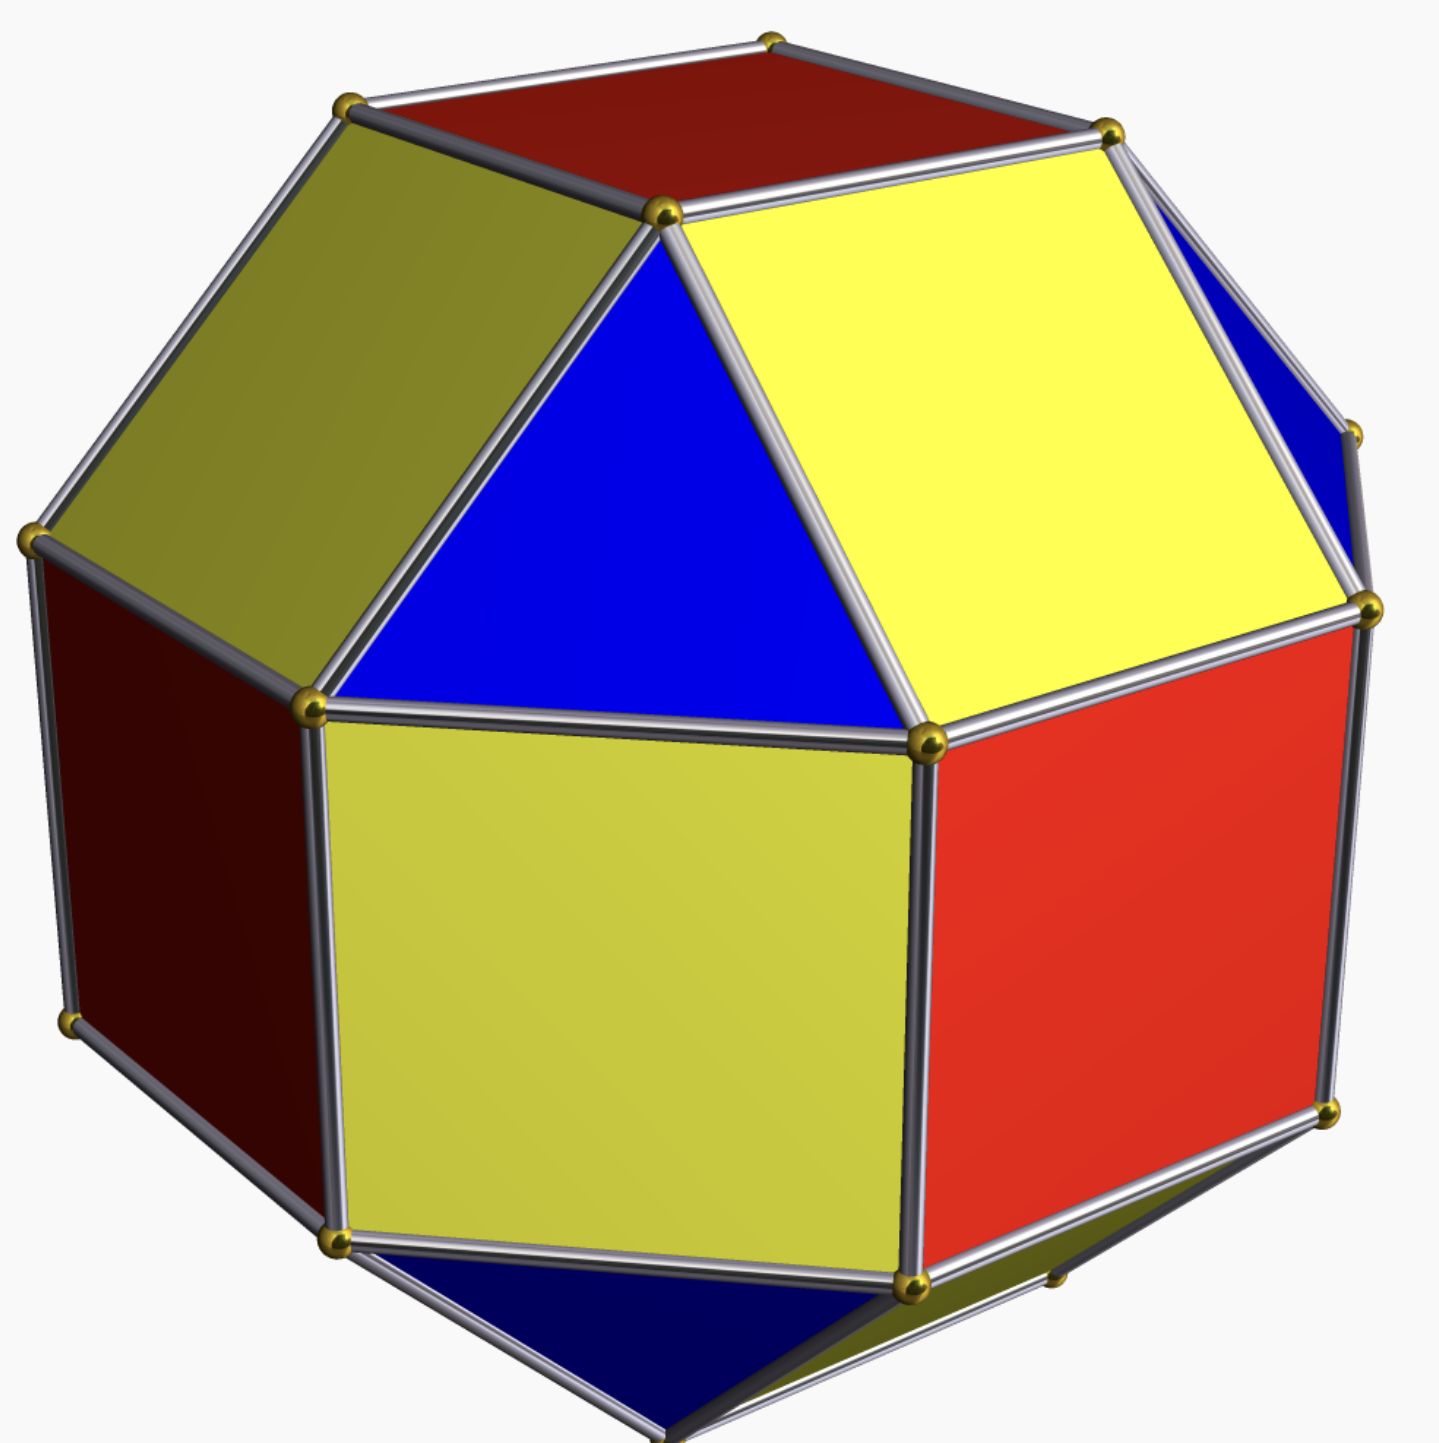
\includegraphics[width=\linewidth]{images/polyeder/Rhombenkuboktaeder.png}
        \caption{Rhombenkuboktaeder.}
        \label{fig:Rhombenkuboktaeder}
    \end{subfigure}
    \hfill
    \begin{subfigure}[b]{0.32\textwidth}
        \centering
        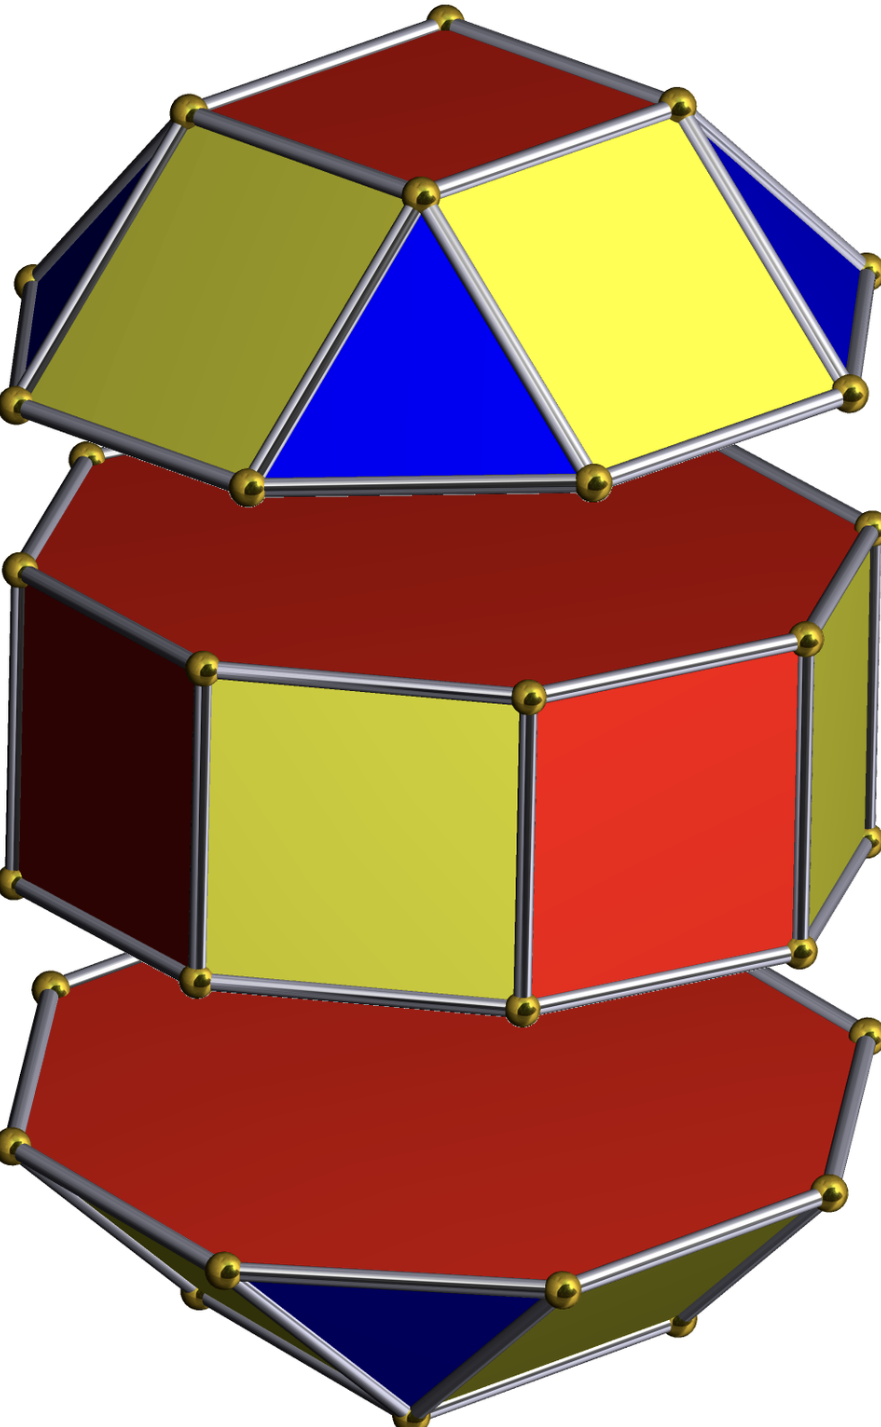
\includegraphics[width=\linewidth]{images/polyeder/RhombenkuboktaederToPseudorhombicuboctahedron.png}
        \caption{Rhombenkuboktaeder zerlegt in ein Prisma und zwei Dome.}
        \label{fig:RhombenkuboktaederZerlegt}
    \end{subfigure}
    \hfill
    \begin{subfigure}[b]{0.32\textwidth}
        \centering
        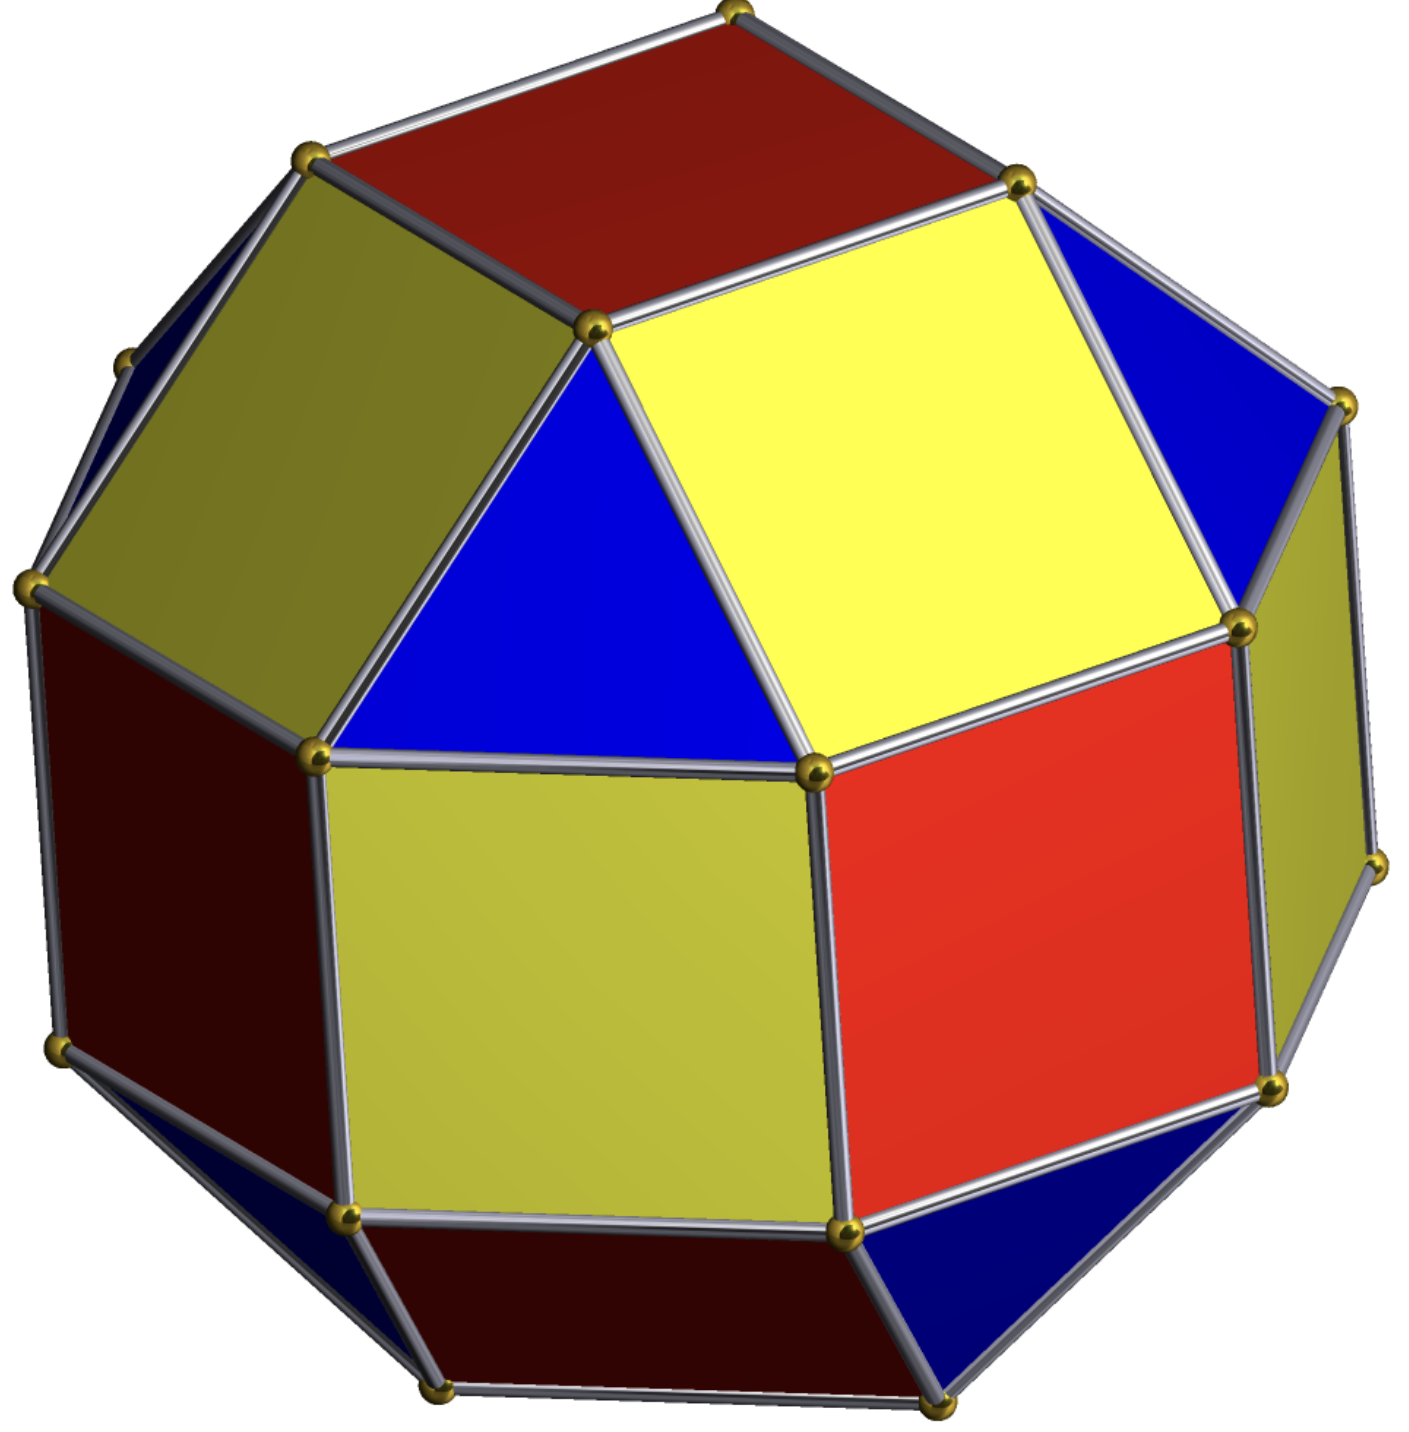
\includegraphics[width=\linewidth]{images/polyeder/Pseudorhombicuboctahedron.png}
        \caption{Pseudo-Rhombenkuboktaeder.}
    \end{subfigure}
    \caption{Rhombenkuboktaeder zu Pseudo-Rhombenkuboktaeder, Wikipedia \cite{elongated_square_gyrobicupola}.}
    \label{fig:rhombenkuboktaederToPseudorhombicuboctahedron}
\end{figure}



\section{Reflexion}

Ein besonderes Merkmal dieses Themas ist seine visuelle Anziehungskraft. Die Untersuchung von Projektionen hochsymmetrischer Körper bietet eine unmittelbare, ästhetische Zugänglichkeit. Obwohl die zugrundeliegende Mathematik – mit Symmetriegruppen, Matrixalgebra und Orthogonalprojektionen – ein sehr hohes und abstraktes Anforderungsniveau besitzt, verhindert die visuelle Aufarbeitung, dass die Theorie trocken wirkt, und bietet einen sehr konkreten Zugang zur Materie. Diese Dualität macht es zu einem äußerst dankbaren Thema: Die Lernenden oder Lesenden können die abstrakten algebraischen Beweise durch die geometrischen Projektionsbilder (wie die Umrisse des Oktaeders) stets kontrollieren und verifizieren. Hier wäre wahrscheinlich auch das grösste Potential vorhanden gewesen, um digitale Medien gezielter einzusetzen. Dieses Thema bietet sich sehr dazu an visuell zu arbeiten und verschiedene Medien, wie Grafiken, Applets, Videos, einzusetzen, um die Dinge zu visualisieren.
\newline
\newline
Zwar ist das vorliegende Skript bewusst in einem sehr formalen, mathematisch rigorosen Stil verfasst und dementsprechend anspruchsvoll, nichtsdestotrotz schließt dies eine Behandlung im gymnasialen Unterricht keinesfalls aus. Im Gegenteil: Gerade durch die hohe visuelle Zugänglichkeit lässt sich die komplexe Theorie gut auf ein greifbares Niveau herunterbrechen. Während für das vollständige Durchdringen der algebraischen Beweise eine gewisse mathematische Reife erforderlich ist, sind die geometrischen Kernaussagen intuitiv erfassbar und können auch auf gymnasialer Stufe problemlos verstanden werden.  
\newline
\newline
Das Thema bietet zudem die seltene Gelegenheit, tiefgreifende lineare Algebra mit einem handlungsorientierten Ansatz zu verknüpfen. Die Möglichkeit, die untersuchten Polyeder (wie die platonischen Körper oder das (Pseudo-)Rhombenkuboktaeder) selbst aus Papier oder Modellbausätzen zu basteln, schlägt eine Brücke zur haptischen Erfahrung. Somit könnte dieses Thema auch Schülerinnen und Schüler (SuS) ansprechen, die ansonsten keinen großen Bezug zur klassischen, rein kalkülbasierten Schulmathematik haben. 
\newline
\newline
Im klassischen Mathematikstudium werden Lineare Algebra und Geometrie häufig sehr isoliert voneinander gelehrt. Lineare Algebra verbleibt oft in abstrakten Vektorräumen, während sich dieses Thema genau an der Schnittmenge bewegt. Es zeigt eindrucksvoll auf, welche enorme geometrische Aussagekraft algebraische Werkzeuge (Symmetrische Matrizen, Diagonalisierbarkeit, Eigenwerte) haben. Ein weiterer didaktisch wertvoller Aspekt der Arbeit ist der starke Bezug zur Darstellenden Geometrie, einem Fachbereich, der in den aktuellen Schul-Curricula oftmals in den Hintergrund geraten ist. Wenn auch anspruchsvoll, kann dieses Thema als eine Weiterführung in diesem Zusammenhang behandelt oder erwähnt werden.
\newline
\newline
Zuletzt bietet das Thema ein reiches Potenzial für die Integration der Mathematikgeschichte. Die Faszination für hochsymmetrische Körper reicht von den antiken Philosophen (Platonische Körper) über Archimedes bis hin zu Johannes Kepler, der diese Formen in seinem kosmologischen Modell des Sonnensystems nutzte. Gleichzeitig spannt das Pseudo-Rhombenkuboktaeder den Bogen in die Moderne, da es erst im 20. Jahrhundert im Rahmen der Johnson-Körper systematisch Beachtung fand. Diese historische Dimension verleiht der Mathematik ein menschliches, kulturelles Gesicht und zeigt, dass die Geometrie ein stetig wachsendes, lebendiges Forschungsfeld ist.
% Bibliography
\bibliographystyle{alpha}
\bibliography{sample}

\end{document}